% small.tex
\documentclass{beamer}
\usetheme{default}
\usepackage{amsmath, amsfonts, amssymb, amsthm, pstricks, pgf,color,tikz}
\usetikzlibrary{arrows,shapes}


% shared
\newenvironment{frcseries}{\fontfamily{frc}\selectfont}{}
\newcommand{\textfrc}[1]{{\frcseries#1}}
\newcommand{\mathfrc}[1]{\raisebox{-0.8mm}{\text{\textfrc{\small #1}}}\hspace{0.4mm}}
\newcommand{\eqn}[1]{\begin{align*}
#1
\end{align*}}
\newcommand{\eqnl}[2]{\begin{align} \label{#1}
#2
\end{align}}
\newcommand{\vect}[1]{\boldsymbol{\mathbf{#1}}}
\newcommand{\degree}[1]{${#1}^{\circ}$}
\newcommand{\highlight}{ \rowcolor{lightgrass} }
\newcommand{\script}[1]{\mathcal{#1}}
\newcommand{\bl}{\big\{}
\newcommand{\br}{\big\}}
\newcommand{\Bl}{\Big\{}
\newcommand{\Br}{\Big\}}
\newcommand{\argmax}{\operatornamewithlimits{argmax}}
\newcommand{\eqnset}[4]{
\[ #1 = #2 \left\{ \begin{array}{#3}
        #4
\end{array} \right. \] 
}
\definecolor{lemonchiffon}{rgb}{1, .98, .80}
\definecolor{lightgrass}{rgb}{.89, 1, .87}
\newcommand{\clr}[2]{{\color{#1}{#2}}}
\newcommand{\indicator}{\mathbf{1}}
\newcommand{\leftlbl}[1]{\mbox{#1} \;\;\;\;\;\;}
\newcommand{\eqnsep}{,\;\;\;\;\;\;\;\;}


% custom
\newcommand{\afe}{\frac{\alpha}{Fe}}
\newcommand{\feh}{\frac{Fe}{H}}
\newcommand{\vz}{\vect{z}}
\newcommand{\vx}{\vect{x}}
\newcommand{\vy}{\vect{y}}
\newcommand{\vp}{\vect{\pi}}
\newcommand{\vph}{\hat{\vect{\pi}}}
\newcommand{\vpmle}{\hat{\vect{\pi}}_\text{MLE}}
\newcommand{\sumn}{\sum^n_{i=1}}
\newcommand{\summ}{\sum^m_{j=1}}
\newcommand{\summo}{\sum^{m-1}_{j=1}}
\newcommand{\sumg}{\sum^g_{j=1}}
\newcommand{\sumk}{\sum^m_{k=1}}
\newcommand{\fab}{f_j}

\newcommand{\vpg}{\vp^{\prime}}
\newcommand{\vpgh}{\hat{\vp}^{\prime}}
\newcommand{\llp}{\mathfrc{l}(\vect{\pi})}
\newcommand{\llpph}{\mathfrc{l}(\vpgh)}
\newcommand{\llpp}{\mathfrc{l}(\vpg)}




\begin{document}
% For every picture that defines or uses external nodes, you'll have to
% apply the 'remember picture' style. To avoid some typing, we'll apply
% the style to all pictures.
\tikzstyle{every picture}+=[remember picture]

% By default all math in TikZ nodes are set in inline mode. Change this to
% displaystyle so that we don't get small fractions.
\everymath{\displaystyle}











%%%%%%%%%%%%%%%%%%%%%%%%%%%%%%%%%%%%%%%%%%%%%%%%%%%%%%%%%%%%%%%
%%%%%%%%%%%%%%%%%%%%%%%%%%%%%%%%%%%%%%%%%%%%%%%%%%%%%%%%%%%%%%%
\begin{frame}{A generative finite mixture model}
	
	
		
	\begin{figure}
			\begin{center}
				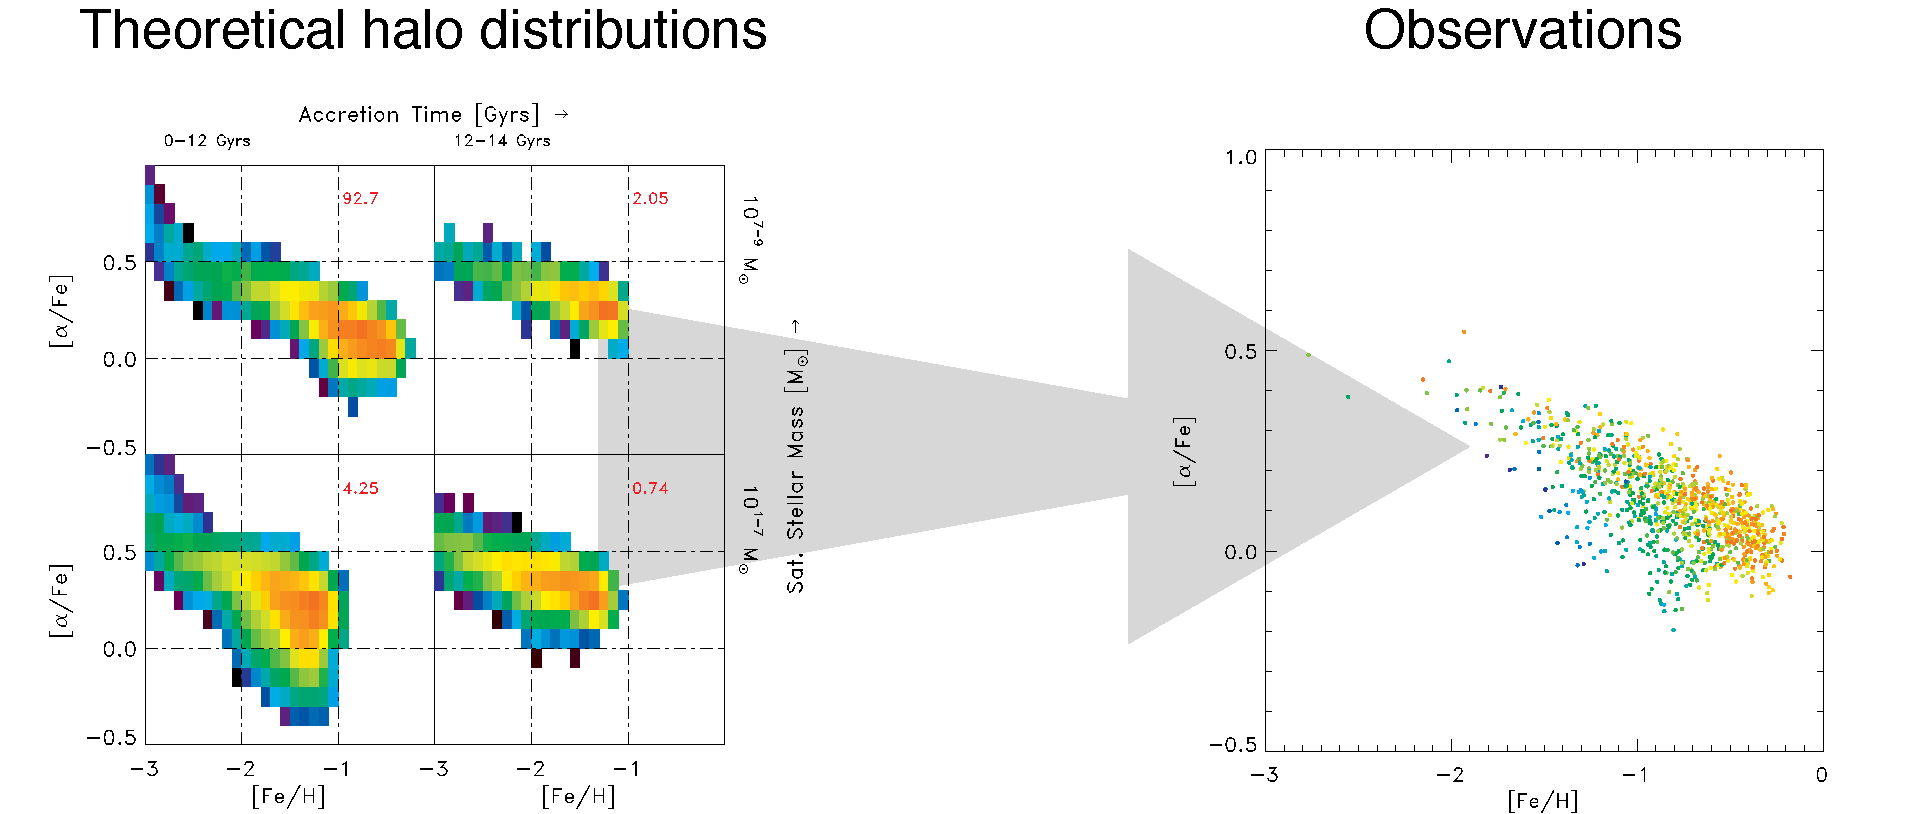
\includegraphics[scale=0.31]{denstoobs.pdf}
			\end{center}
	\end{figure}
	
	\vspace{-8mm}
	
	\eqn{
		\Bigg[\feh,\afe\Bigg]_{i=1}^{N} \text{i.i.d} \sim f(x,y) = \sum^m_{j=1} \pi_j f_j(x,y)
	}
	
	\begin{center}
		Where the mixing proportions, $\vp$, give the formation history.
	\end{center}
	
\end{frame}
%---------------------------------------------------------------------------------------------------------------------------------------------------------------------------
\begin{frame}[shrink]{A generative finite mixture model}
	
	\begin{itemize}
		
		
		\item each observed point comes from one of $m$ mixture components (pictured)
		\item we propose a generative model in the form of a finite mixture model
		\item since each mixture component has an associated mass and accretion time range, the formation history is specified if we know what percentage of observations come from each mixture component
		\item our goal, then, is to determine the mixing proportions, $\vp$
		
		\item note that the simulations that produce observed points do not follow this model; we don't know the true generative method, and are proposing a reasonable one that we think can be fit, and that will spit out the formation history
	\end{itemize}
	
\end{frame}







%%%%%%%%%%%%%%%%%%%%%%%%%%%%%%%%%%%%%%%%%%%%%%%%%%%%%%%%%%%%%%%
%%%%%%%%%%%%%%%%%%%%%%%%%%%%%%%%%%%%%%%%%%%%%%%%%%%%%%%%%%%%%%%
\begin{frame}{Model definition}
	
	\eqn{
		\leftlbl{Let} x=\afe \eqnsep y=\feh
	 }
	
	Given $m$ mixture components, we propose that the density from which observations are generated is
	
	\begin{equation}
		f(x,y) = \sum^m_{j=1}
		\tikz[baseline]{\node[fill=blue!20,anchor=base] (t3) {$\pi_j$};}
		\tikz[baseline]{\node[fill=red!20,anchor=base] (t4) {$f_j(x,y)$};}
	\end{equation}
	\begin{itemize}
		\item
		Mixing proportion \tikz\node[fill=blue!20,draw,circle] (n3){};
		\item
		Mixture component $j$ \tikz\node[fill=red!20,draw,circle] (n4){};
	\end{itemize}
		
	\begin{tikzpicture}[overlay]
		\path[->] (n3) edge [out=0, in=-90] (t3);
		\path[->] (n4) edge [out=0, in=-90] (t4);
	\end{tikzpicture}
	
	
	
	
	
	
	\eqn{
		\leftlbl{where} \sum^m_{j=1} \pi_j = 1 \eqnsep   \pi_j \geq 0  \eqnsep   j=1,\ldots,m
	 }
	
\end{frame}
%---------------------------------------------------------------------------------------------------------------------------------------------------------------------------
\begin{frame}[shrink]{Definitions}
	
	\begin{itemize}
		\item For notational simplicity, x=$\afe$ and y=$\feh$
		\item Formally, given m mixture components, the density from which all observations are drawn is as shown
		\item The mixing proportions, $\vp$ must be non-negative, and sum to 1
	\end{itemize}
	
\end{frame}

















%%%%%%%%%%%%%%%%%%%%%%%%%%%%%%%%%%%%%%%%%%%%%%%%%%%%%%%%%%%%%%%
%%%%%%%%%%%%%%%%%%%%%%%%%%%%%%%%%%%%%%%%%%%%%%%%%%%%%%%%%%%%%%%
\begin{frame}{Estimating the mixing proportions $\vect{\pi}$}
	
	To estimate the mixing proportions, we can use a maximum likelihood approach
	\eqn{
		\vph_{\text{MLE}} &= \argmax_{\vp} L(\vect{\pi})
	}
	
	
	
	\eqn{
		\leftlbl{where} \script{L}(\vect{\pi}) &= \sumn \log \Big( \summ \pi_j \fab(x_i,y_i)  \Big)
	}
	
	Unfortunately the standard MLE procedure for estimating $\vp$ is intractable with this likelihood.\newline
	
	Expectation Maximization (EM) algorithm to the rescue!
	
	
	
\end{frame}
%---------------------------------------------------------------------------------------------------------------------------------------------------------------------------
\begin{frame}[shrink]{Estimating the mixing proportions $\vect{\pi}$}
	
	\begin{itemize}
		\item hi
	\end{itemize}
	
\end{frame}

















%%%%%%%%%%%%%%%%%%%%%%%%%%%%%%%%%%%%%%%%%%%%%%%%%%%%%%%%%%%%%%%
%%%%%%%%%%%%%%%%%%%%%%%%%%%%%%%%%%%%%%%%%%%%%%%%%%%%%%%%%%%%%%%
\begin{frame}{Expectation Maximization}
	
	Suppose we knew which mixture component $f_j$ each observation came from:
	
	\eqnset{z_{ij} = \indicator(x_i,y_i \sim f_j) }{}{ll}{
		1			& (x_i,y_i) \sim f_j 		\\
		0		& \text{otherwise}
	}
	
	The log likelihood can then be expressed as
	
	\eqn{
		\llp &= \sumn \summ z_{ij}  \log \bl \pi_j  \fab(x_i,y_i) \br
	}
	
	The addition of the latent variable $\vect{z}$ actually makes things easier because it is easily differentiable in $\vp$.
	
\end{frame}
%---------------------------------------------------------------------------------------------------------------------------------------------------------------------------
\begin{frame}[shrink]{Expectation Maximization}
	
	\begin{itemize}
		\item Suppose we knew which mixture component $f_j$ each observation came from
		\item Then we could construct a latent indicator variable, $z_{ij}$, which is 1 if point $i$ comes from mixture component $j$, and 0 otherwise
		\item The log like then becomes
		\item Since we're supposing that we know $z_{ij}$, it's trivial to differentiate this log likelihood with respect to $\vph$
		\item 
	\end{itemize}
	
\end{frame}










%%%%%%%%%%%%%%%%%%%%%%%%%%%%%%%%%%%%%%%%%%%%%%%%%%%%%%%%%%%%%%%
%%%%%%%%%%%%%%%%%%%%%%%%%%%%%%%%%%%%%%%%%%%%%%%%%%%%%%%%%%%%%%%
\begin{frame}{Estimating $\vph$ using expectation maximization}
	
	We don't know $\vect{z}$, so we replace $\vect{z}$ with the expected value of $\vect{z}$, conditioned on the data and the last known $\vph$:
	
	%Expectation Maximization replaces the unobservable $\vect{z}$ with the expected value of $\vect{z}$, conditional on the data
	
	\eqn{
		\vph^{(t)} &= \argmax_{\vp} \mathbb{E}\Big[\llp \big| \vx,\vy,\vph^{(t-1)} \Big]   
	}
	
	Starting with some random initial value for $\vph^{(0)}$, we iteratively
	
	\begin{itemize}
		\item Find the expected value of $\llp$ using the current expected values of the latent variable $\vect{z}$
		\item Set $\vph^{(t)}$ to the $\argmax_{\vp}$ of this expectation, which is simple to compute
	\end{itemize}
	
	And repeat until $\llp$ stabilizes to a range  $< 10^{-4}$
	
	
	
\end{frame}
%---------------------------------------------------------------------------------------------------------------------------------------------------------------------------
\begin{frame}[shrink]{Estimating the mixing proportions $\vect{\pi}$}
	
	\begin{itemize}
		\item We don't know $\vect{z}$, so we replace $\vect{z}$ with the expected value of $\vect{z}$, conditioned on the data and the last known $\vph$:
		\item 
		\item the true likelihood is increasing in each iteration
	\end{itemize}
	
\end{frame}








%%%%%%%%%%%%%%%%%%%%%%%%%%%%%%%%%%%%%%%%%%%%%%%%%%%%%%%%%%%%%%%
%%%%%%%%%%%%%%%%%%%%%%%%%%%%%%%%%%%%%%%%%%%%%%%%%%%%%%%%%%%%%%%
\begin{frame}{Find the expected value of $L(\vect{\pi})$ using the current expected value of the latent variable}
	
	The expected value of $\llp$, with respect to the conditional distribution of $\vect{z}$, given observed data and $\vp^{(t-1)}$ is
	
	\eqn{
		\mathbb{E}_{\vp}\Big[\llp \big| \vx,\vy \Big] &= \sumn \summ \mathbb{E}_{\vp}\big[z_{ij}|x_i,y_i\big] \bl \log \fab(x_i,y_i) + \log \pi_j  \br
	}
	
	Since $z_{ij}$ is an indicator, its expected value is simply the probability that data point $i$ comes from model $j$
	\eqn{
		\mathbb{E}_{\vp}\Big[  z_{ij} | x_i, y_i \Big]	&= \text{Pr}_{\vp}(z_{ij}|x_i,y_i)	\\
										&= \frac{p(x_i,y_i|z_{ij}=1)p(z_{ij}=1)}{p(x_i,y_i)}	\\
										&=  \frac{\pi_j \fab(x_i,y_i)  }{\summ \pi_j \fab(x_i,y_i)}
	}
\end{frame}
%---------------------------------------------------------------------------------------------------------------------------------------------------------------------------
\begin{frame}[shrink]{Find the expected value of $L(\vect{\pi})$ using the current expected value of the latent variable}
	
	\begin{itemize}
		\item cond prob
	\end{itemize}
	
\end{frame}














%%%%%%%%%%%%%%%%%%%%%%%%%%%%%%%%%%%%%%%%%%%%%%%%%%%%%%%%%%%%%%%
%%%%%%%%%%%%%%%%%%%%%%%%%%%%%%%%%%%%%%%%%%%%%%%%%%%%%%%%%%%%%%%
\begin{frame}{Find the $\argmax_{\vp}$ of this expectation}
	
		
	Now that we have the expected value of $\llp$ with respect to the conditional distribution of $\vect{z}$, we need only evaluate
	
	
	\eqn{
		\vph^{(t)} &= \argmax_{\vp} \mathbb{E}\Big[\llp \big| \vx,\vy,\vph^{(t-1)} \Big]   
	}
	
	
	Which can be analytically specified, at each time $t$, as:
	
	\eqn{
		\hat{\pi}^{(t)}_k  = \frac{\sumn w^{(t-1)}_{ij}}{n}
	}
	
	\eqn{
		\leftlbl{where} w^{(t+1)}_{ij} = \frac{\pi^{(t)}_{j} \fab(x_i,y_i)}{\sumk \pi^{(t)}_{k}f_k(x_i,y_i)}	
	}
	

	
\end{frame}
%---------------------------------------------------------------------------------------------------------------------------------------------------------------------------
\begin{frame}[shrink]{Find the $\argmax_{\vp}$ of this expectation}
	
	\begin{itemize}
		\item Note how simple this is to compute
	\end{itemize}
	
\end{frame}





















%%%%%%%%%%%%%%%%%%%%%%%%%%%%%%%%%%%%%%%%%%%%%%%%%%%%%%%%%%%%%%%
%%%%%%%%%%%%%%%%%%%%%%%%%%%%%%%%%%%%%%%%%%%%%%%%%%%%%%%%%%%%%%%
\begin{frame}{Simulations}
	
	
	
	
	\begin{itemize}
		\item Generated observations from 10 realizations of halos
		\item Generated mixing components for these halos
		\item Used a 5x5 grid ($m=25$), and several 2x2 grids ($m=4$)
	\end{itemize}
	
	
	
	\begin{figure}
			\begin{center}
				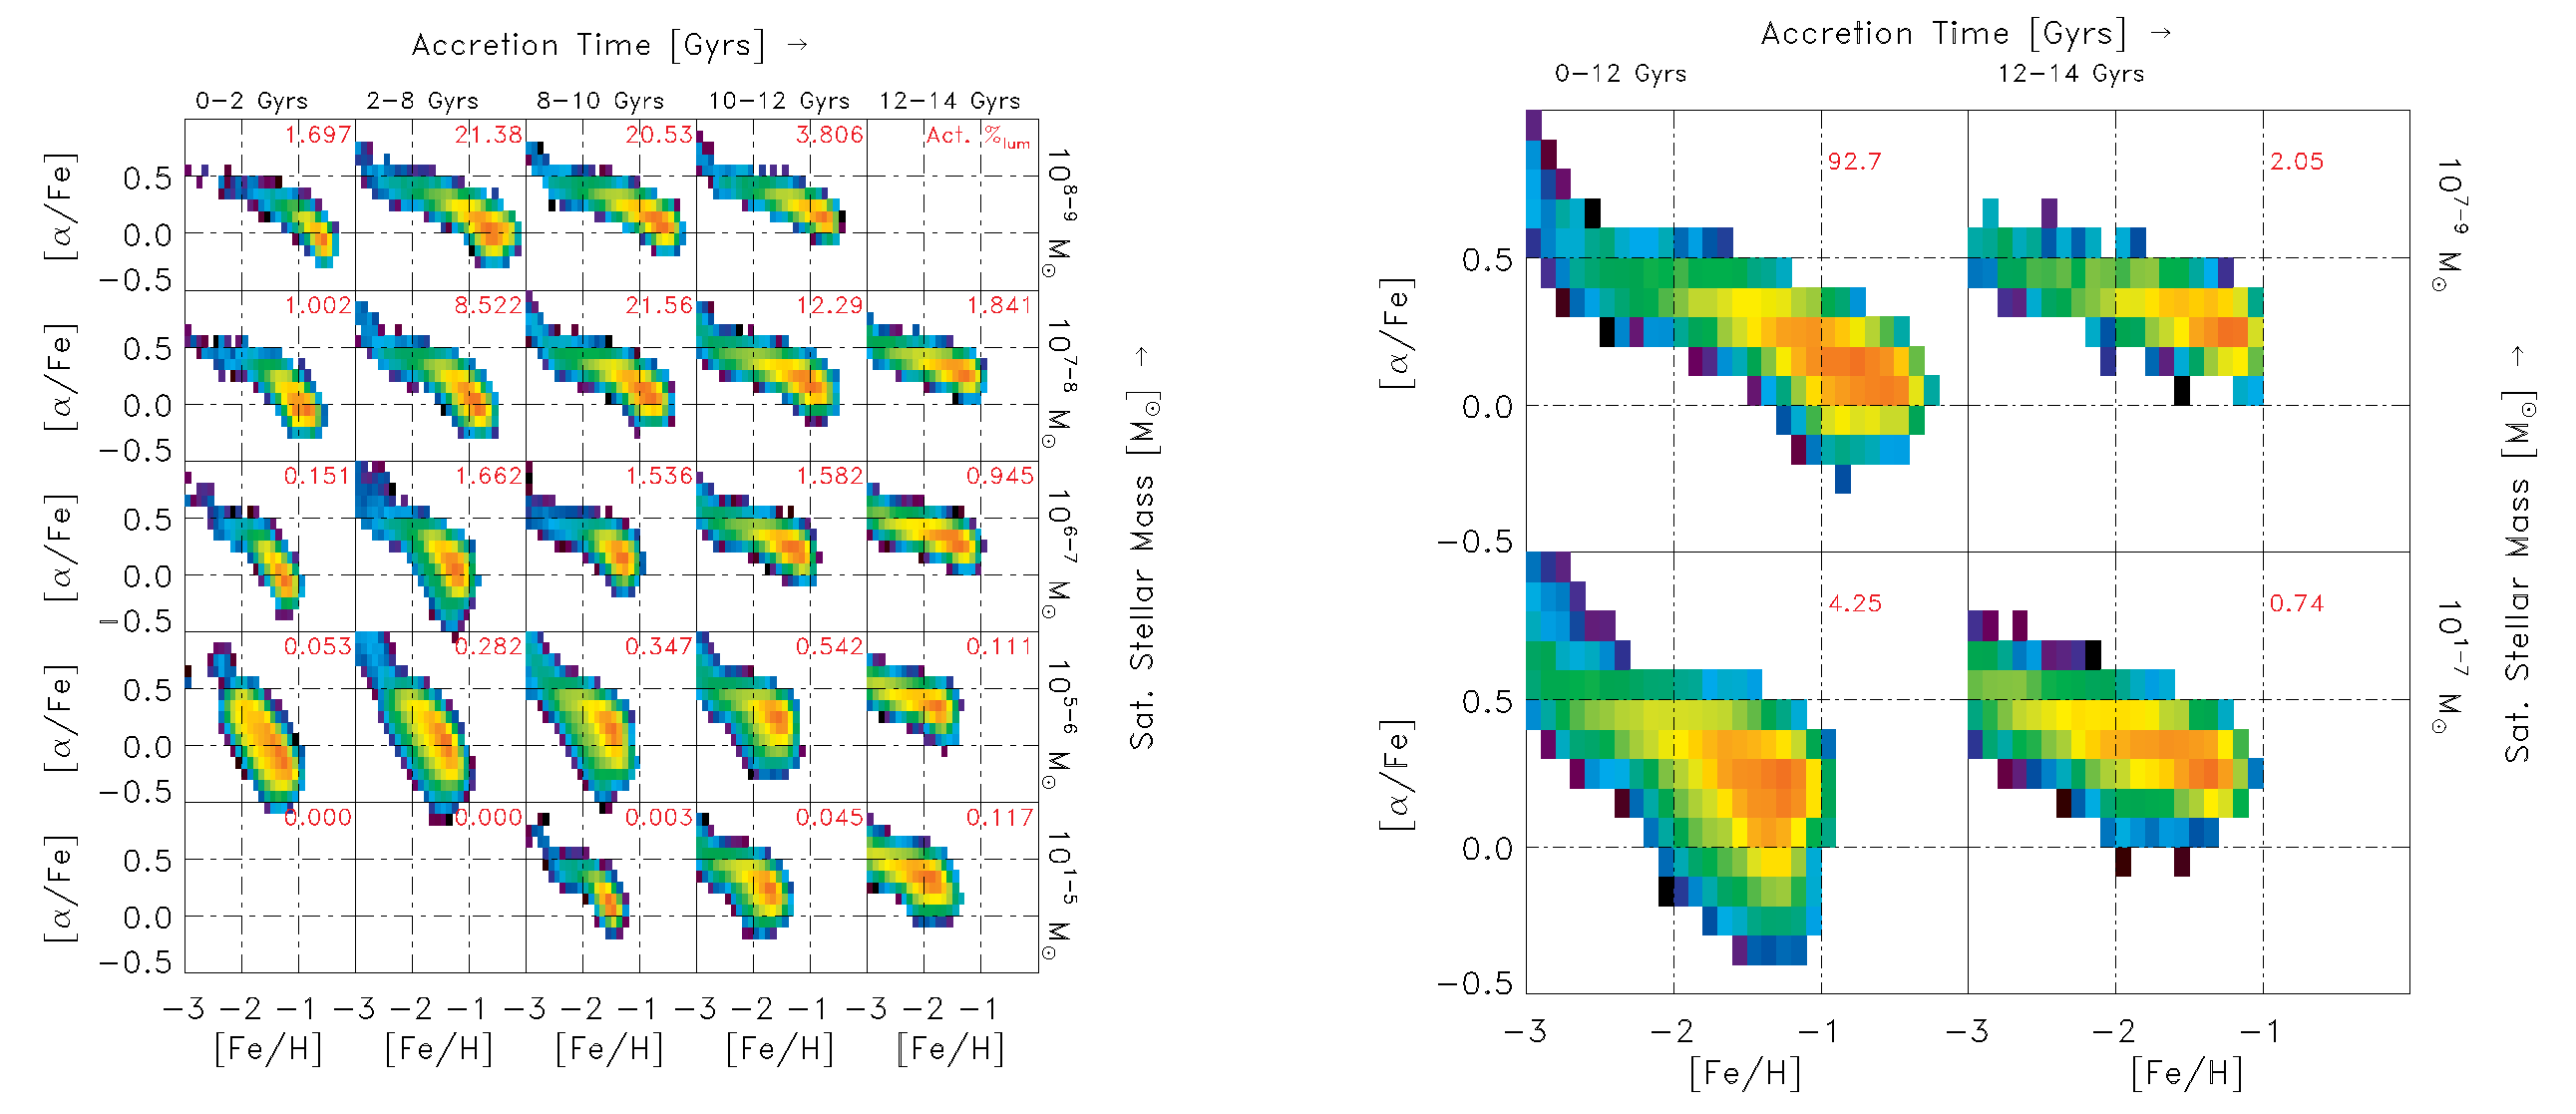
\includegraphics[width=\textwidth]{ourdens.pdf}
			\end{center}
	\end{figure}
	
	
	
	
\end{frame}
%---------------------------------------------------------------------------------------------------------------------------------------------------------------------------
\begin{frame}[shrink]{Simulations}
	
	\begin{itemize}
		\item Tried several different mass/accretion time separations for 2x2
		\item 5x5 grid did not work for some halo realizations
		\item 2x2 grid reliably converged on the correct mixing proportions
		\item since these observations were generated from the simulations (not our model) we know the correct mixing proportions, pi
	\end{itemize}
	
\end{frame}
















%%%%%%%%%%%%%%%%%%%%%%%%%%%%%%%%%%%%%%%%%%%%%%%%%%%%%%%%%%%%%%%
%%%%%%%%%%%%%%%%%%%%%%%%%%%%%%%%%%%%%%%%%%%%%%%%%%%%%%%%%%%%%%%
\begin{frame}{Halo 2: least accurate 2x2 fit}	
	
	\begin{figure}
			\begin{center}
				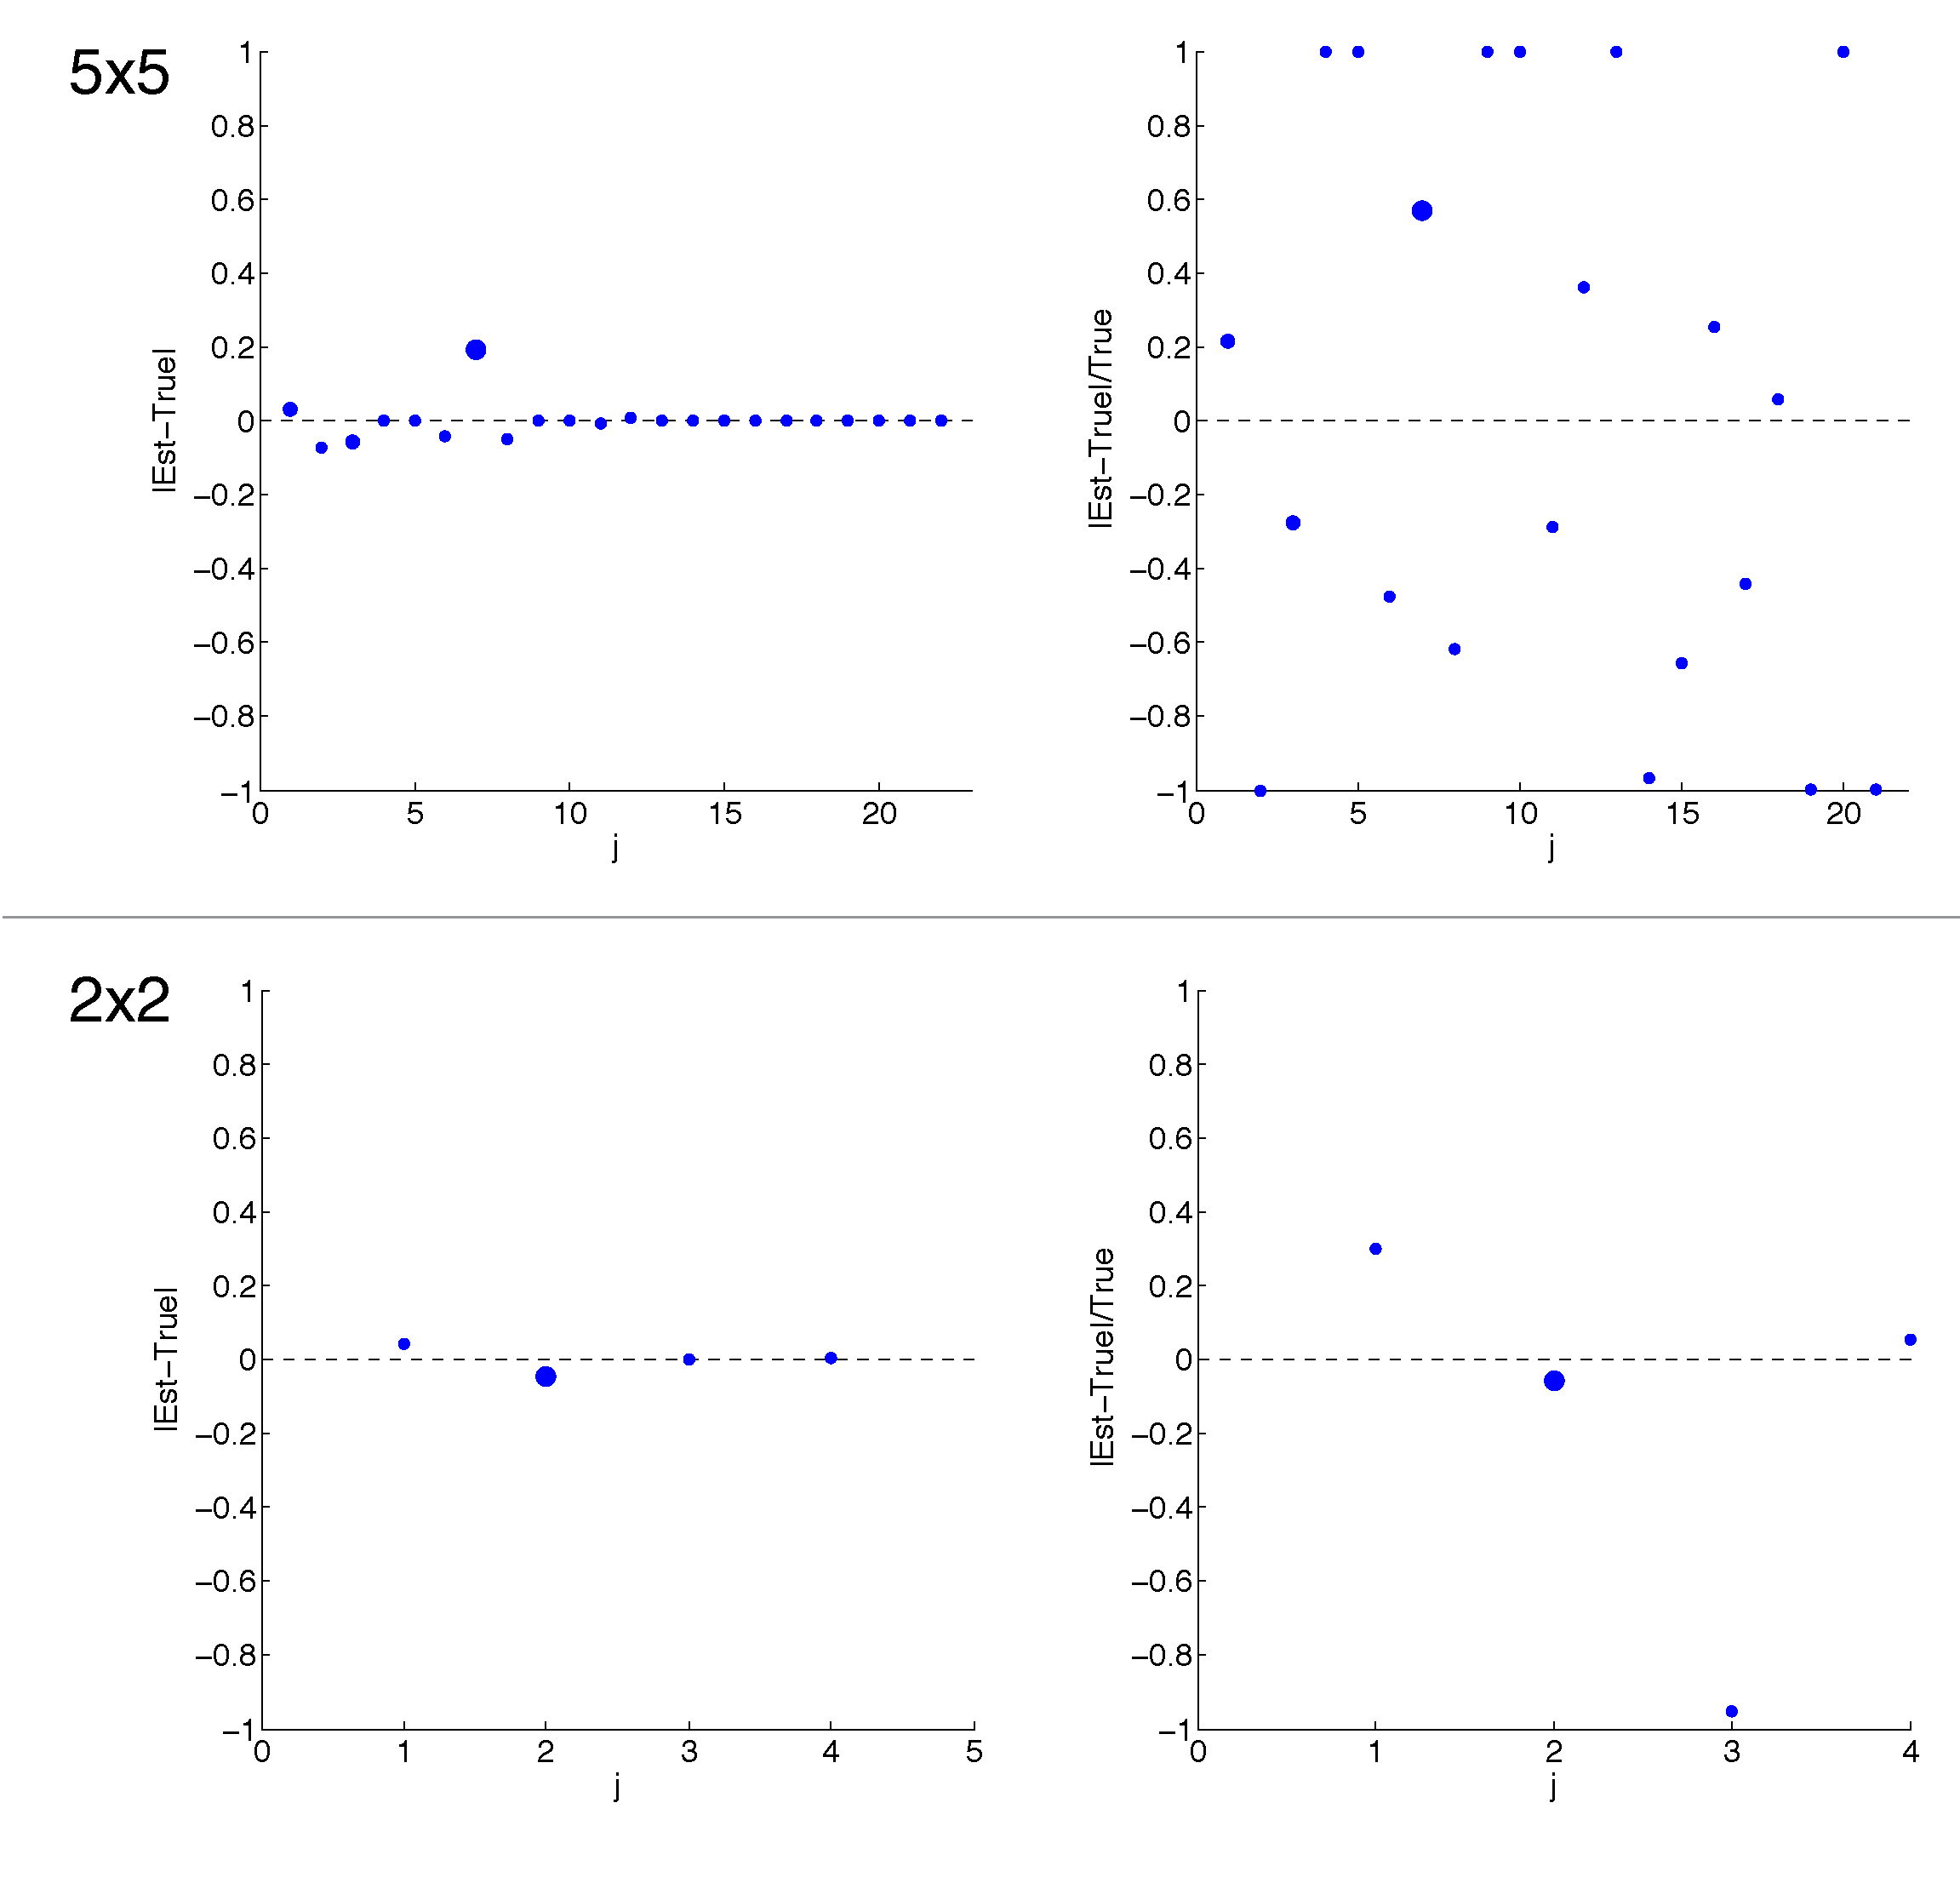
\includegraphics[scale=0.22]{halo2pct2x25x5.pdf}
			\end{center}
	\end{figure}	
	
\end{frame}
%---------------------------------------------------------------------------------------------------------------------------------------------------------------------------
\begin{frame}[shrink]{Halo 2 results}
	
	\begin{itemize}
		\item top is 5x5
		\item bottom is 2x2
		\item left is absolute difference between the true mixing proportions and the estimated ones
		\item right is percent difference between the true mixing proportions and the estimated ones
		\item 2x2 is pretty close, although not a perfect fit, it does reconstruct the formation history fairly accurately.
	\end{itemize}
	
\end{frame}

















%%%%%%%%%%%%%%%%%%%%%%%%%%%%%%%%%%%%%%%%%%%%%%%%%%%%%%%%%%%%%%%
%%%%%%%%%%%%%%%%%%%%%%%%%%%%%%%%%%%%%%%%%%%%%%%%%%%%%%%%%%%%%%%
\begin{frame}{Halo 5: most accurate 2x2 fit}
	
	\begin{figure}
			\begin{center}
				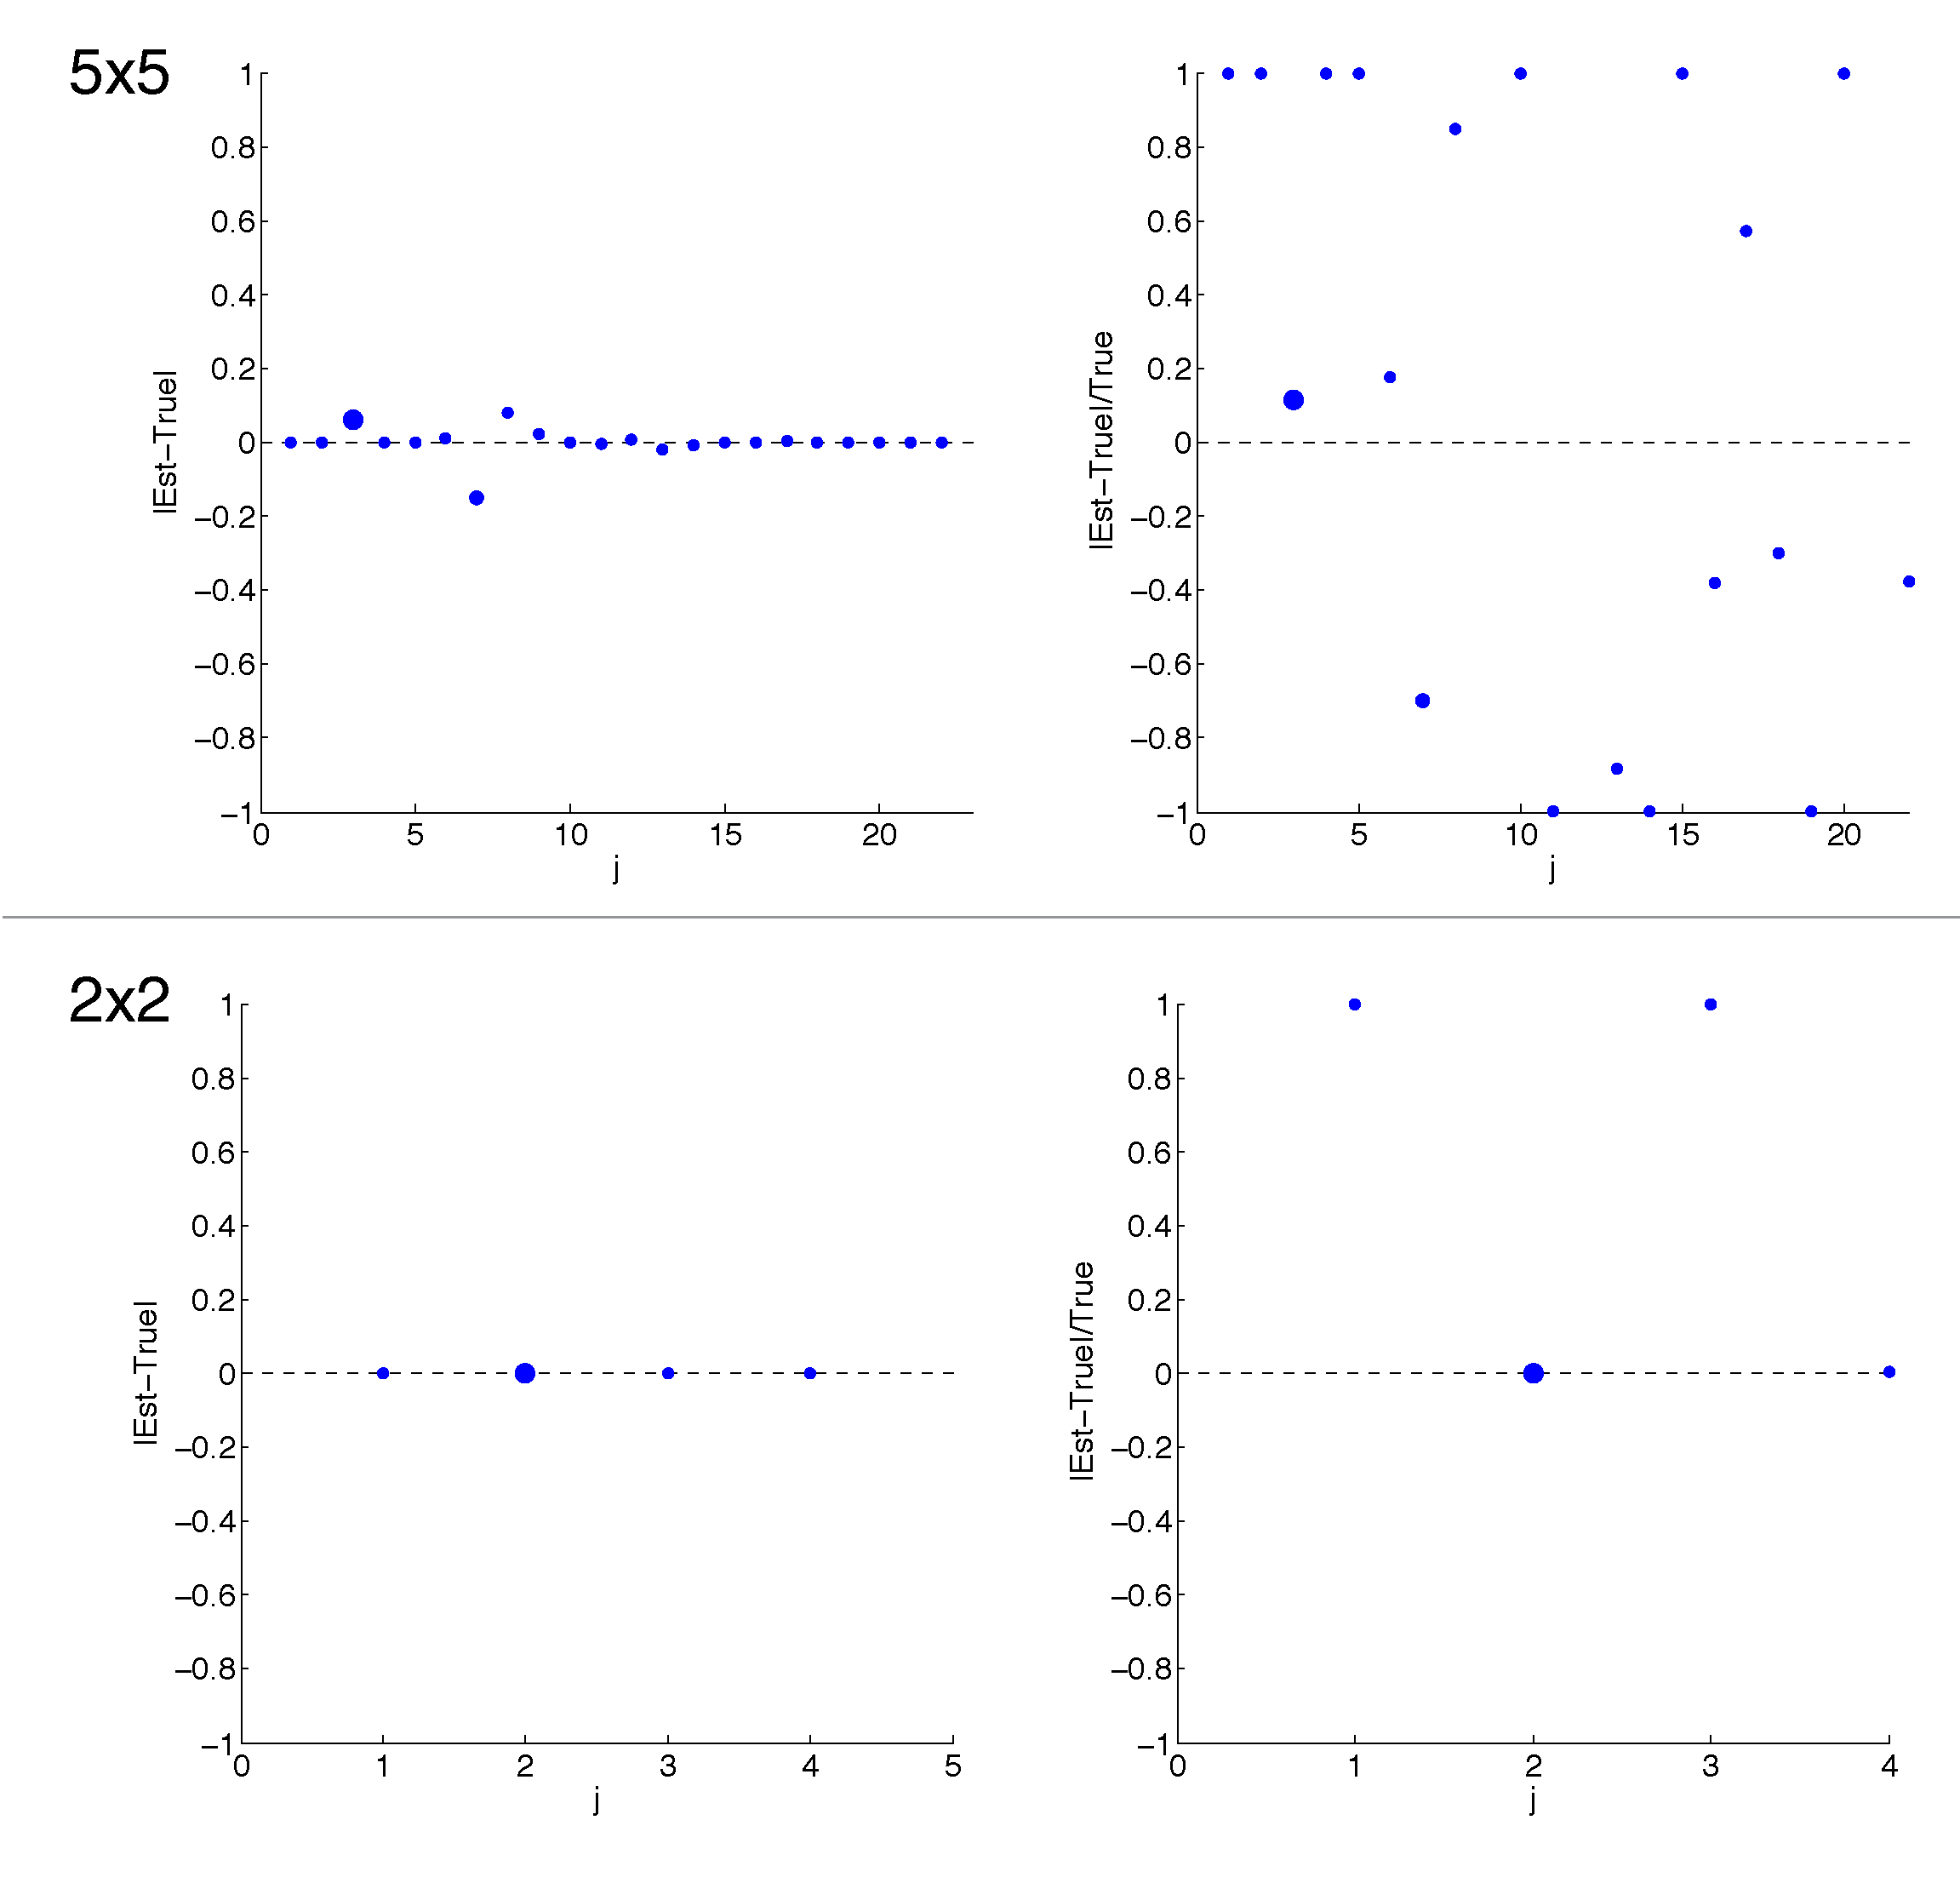
\includegraphics[scale=0.22]{halo5pct2x25x5.pdf}
			\end{center}
	\end{figure}	
	
\end{frame}
%---------------------------------------------------------------------------------------------------------------------------------------------------------------------------
\begin{frame}[shrink]{Halo 5 results}
	
	\begin{itemize}
		\item Running the same algorithm for another halo realization
		\item In this case, the 2x2 is dead-on
		\item The large percent differences are caused by a true value of 0 and an estimated value of $< 1 x 10^{-6}$
		\item In general, the 10 different halo realizations have accuracies falling somewhere in between the good fit pictured here, and the less good fit from the previous slide.

	\end{itemize}
	
\end{frame}

















%%%%%%%%%%%%%%%%%%%%%%%%%%%%%%%%%%%%%%%%%%%%%%%%%%%%%%%%%%%%%%%
%%%%%%%%%%%%%%%%%%%%%%%%%%%%%%%%%%%%%%%%%%%%%%%%%%%%%%%%%%%%%%%
\begin{frame}{2x2: All 10 halos}
	
	\begin{figure}
			\begin{center}
				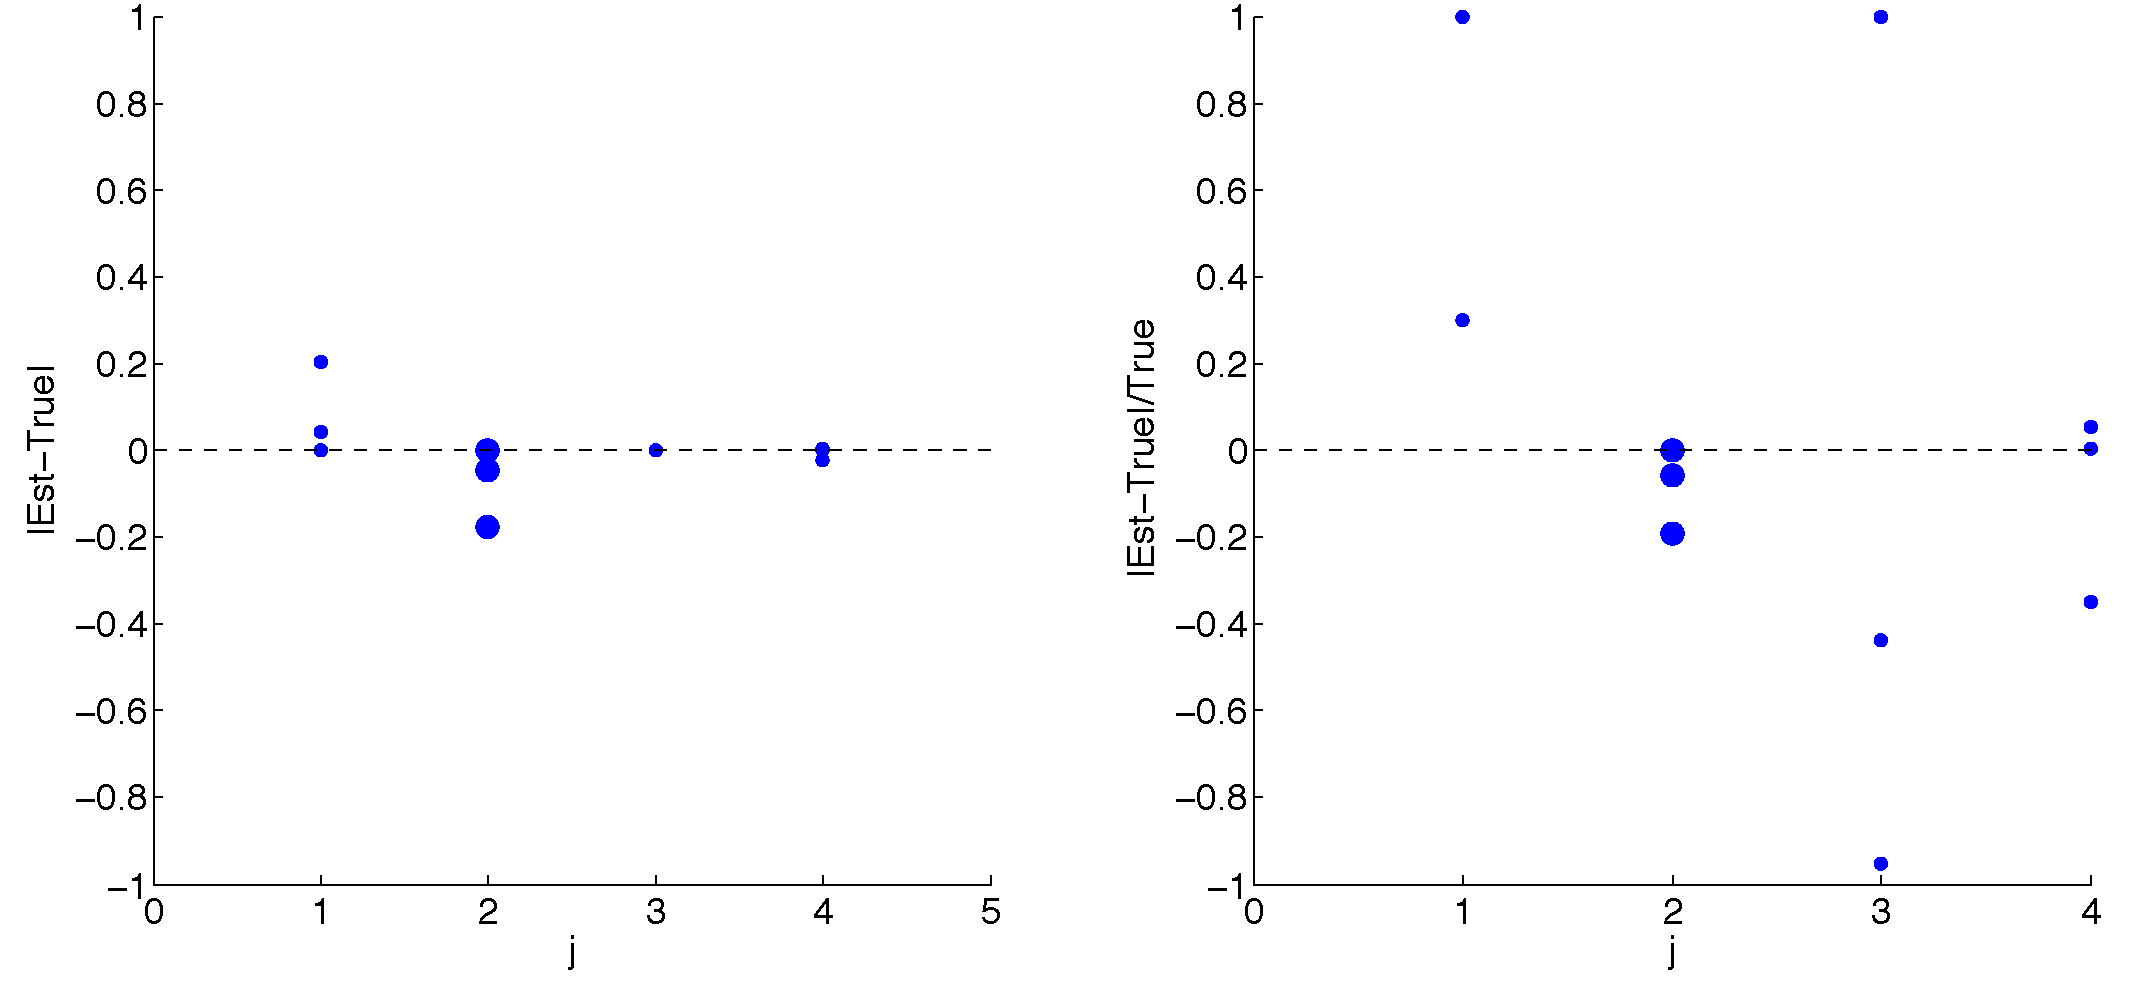
\includegraphics[scale=0.30]{s4t2m7allpctdiff.pdf}
			\end{center}
	\end{figure}	
	
\end{frame}
%---------------------------------------------------------------------------------------------------------------------------------------------------------------------------
\begin{frame}[shrink]{2x2: All 10 halos}
	
	\begin{itemize}
		\item Same graphs, but all 10 halo realizations stacked on top of eachother
		\item In general, the 2x2 reconstructs the formation history fairly well
	\end{itemize}
	
\end{frame}




















%%%%%%%%%%%%%%%%%%%%%%%%%%%%%%%%%%%%%%%%%%%%%%%%%%%%%%%%%%%%%%%
%%%%%%%%%%%%%%%%%%%%%%%%%%%%%%%%%%%%%%%%%%%%%%%%%%%%%%%%%%%%%%%
\begin{frame}{Convergence and minimum observation size}
	
	\begin{figure}
			\begin{center}
				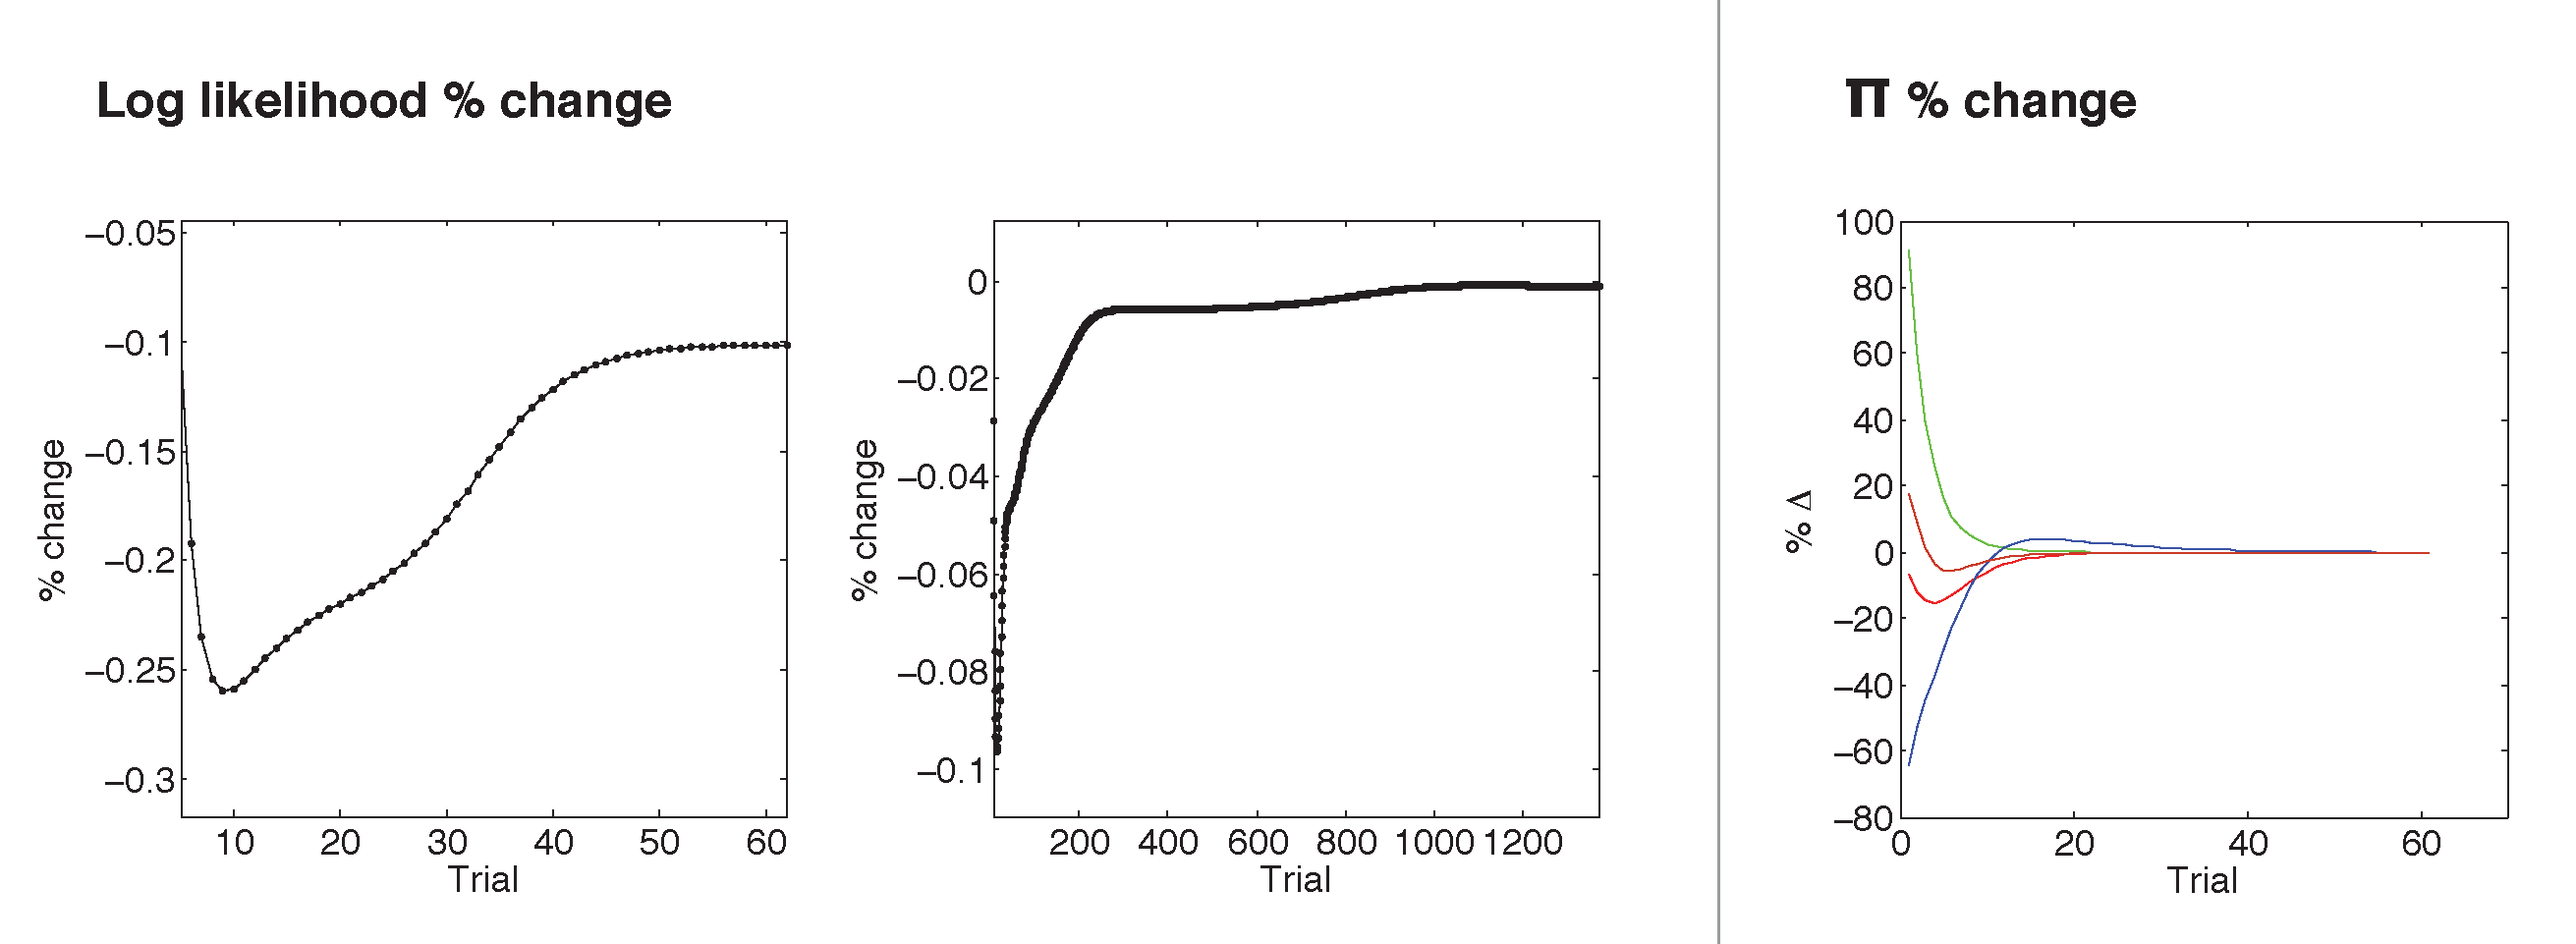
\includegraphics[width=\textwidth]{diag_simple.pdf}
			\end{center}
	\end{figure}
	
	\begin{itemize}
		\item Works with as few as 1,000 observations
		\item Insensitive to initialization of $\vect{\pi}$
		\item Always converges
		\item Large weights identified after 10 iterations
		\item $\llp$ stops changing appreciably after 60 ($m$=4) or 600 ($m$=25) iterations
	\end{itemize}

	
\end{frame}
%---------------------------------------------------------------------------------------------------------------------------------------------------------------------------
\begin{frame}[shrink]{Convergence and minimum observation size}
		
%	1,000 obs, 62 runs, 0.3s m=4
	
%	50,000 obs, 1371 runs, 460s, m=25
	\begin{itemize}
		\item The EM algorithm is not known to converge particularly quickly
		\item For a 2x2 with 1,000 observations, it takes about 60 iterations, or 0.3 seconds, to trigger the stopping condition of less than $10^{-4}$ change in log likelihood
		
		\item since our mixture model is not the true generative model, we can consistently converge on estimates of the mixing proportions that are incorrect.
		\item this happened with 5x5 grids especially, and could be a reflection of over-fitting, or a symptom of too-tight a grid
		\item we did not see any degeneracies--we always converged on the same answers, even if they weren't the "true" values.
		
	\end{itemize}
	
\end{frame}











%%%%%%%%%%%%%%%%%%%%%%%%%%%%%%%%%%%%%%%%%%%%%%%%%%%%%%%%%%%%%%%
%%%%%%%%%%%%%%%%%%%%%%%%%%%%%%%%%%%%%%%%%%%%%%%%%%%%%%%%%%%%%%%
\begin{frame}{Covariance and confidence intervals}
	
	The asymptotic covariance matrix of $\vph$ can be approximated by the inverse of the observed Fisher information matrix, $I$:
	
	\eqn{	
		I(\vpg|\vx,\vy)=-\frac{\partial^2 \llpp}{\partial \vp^\prime \partial \vp^{\prime T}}
	}
	
	
	
	\eqn{
		\text{Cov}(\hat{\pi}_p,\hat{\pi}_q) = \big[I^{-1}(\vpgh) \big]_{pq}
	}
	
	\;\;
	with variance and correlation given by
	
	\eqn{
		\text{Var}(\hat{\pi}_j) &= \sigma^2_j = \Bl  \text{Cov}(\vph) \Br_{jj}
	}
	
	\eqn{
		\text{Corr}(\hat{\pi}_p,\hat{\pi}_q) = \frac{\text{Cov}(\hat{\pi}_p,\hat{\pi}_q)}{\sqrt{\sigma^2_p \sigma^2_q}}
	}
	

	
\end{frame}
%---------------------------------------------------------------------------------------------------------------------------------------------------------------------------
\begin{frame}[shrink]{Covariance and confidence intervals}
	
	\begin{itemize}
		\item 1
	\end{itemize}
	
\end{frame}











%%%%%%%%%%%%%%%%%%%%%%%%%%%%%%%%%%%%%%%%%%%%%%%%%%%%%%%%%%%%%%%
%%%%%%%%%%%%%%%%%%%%%%%%%%%%%%%%%%%%%%%%%%%%%%%%%%%%%%%%%%%%%%%
\begin{frame}{Confidence Intervals}
	
	\begin{figure}
			\begin{center}
				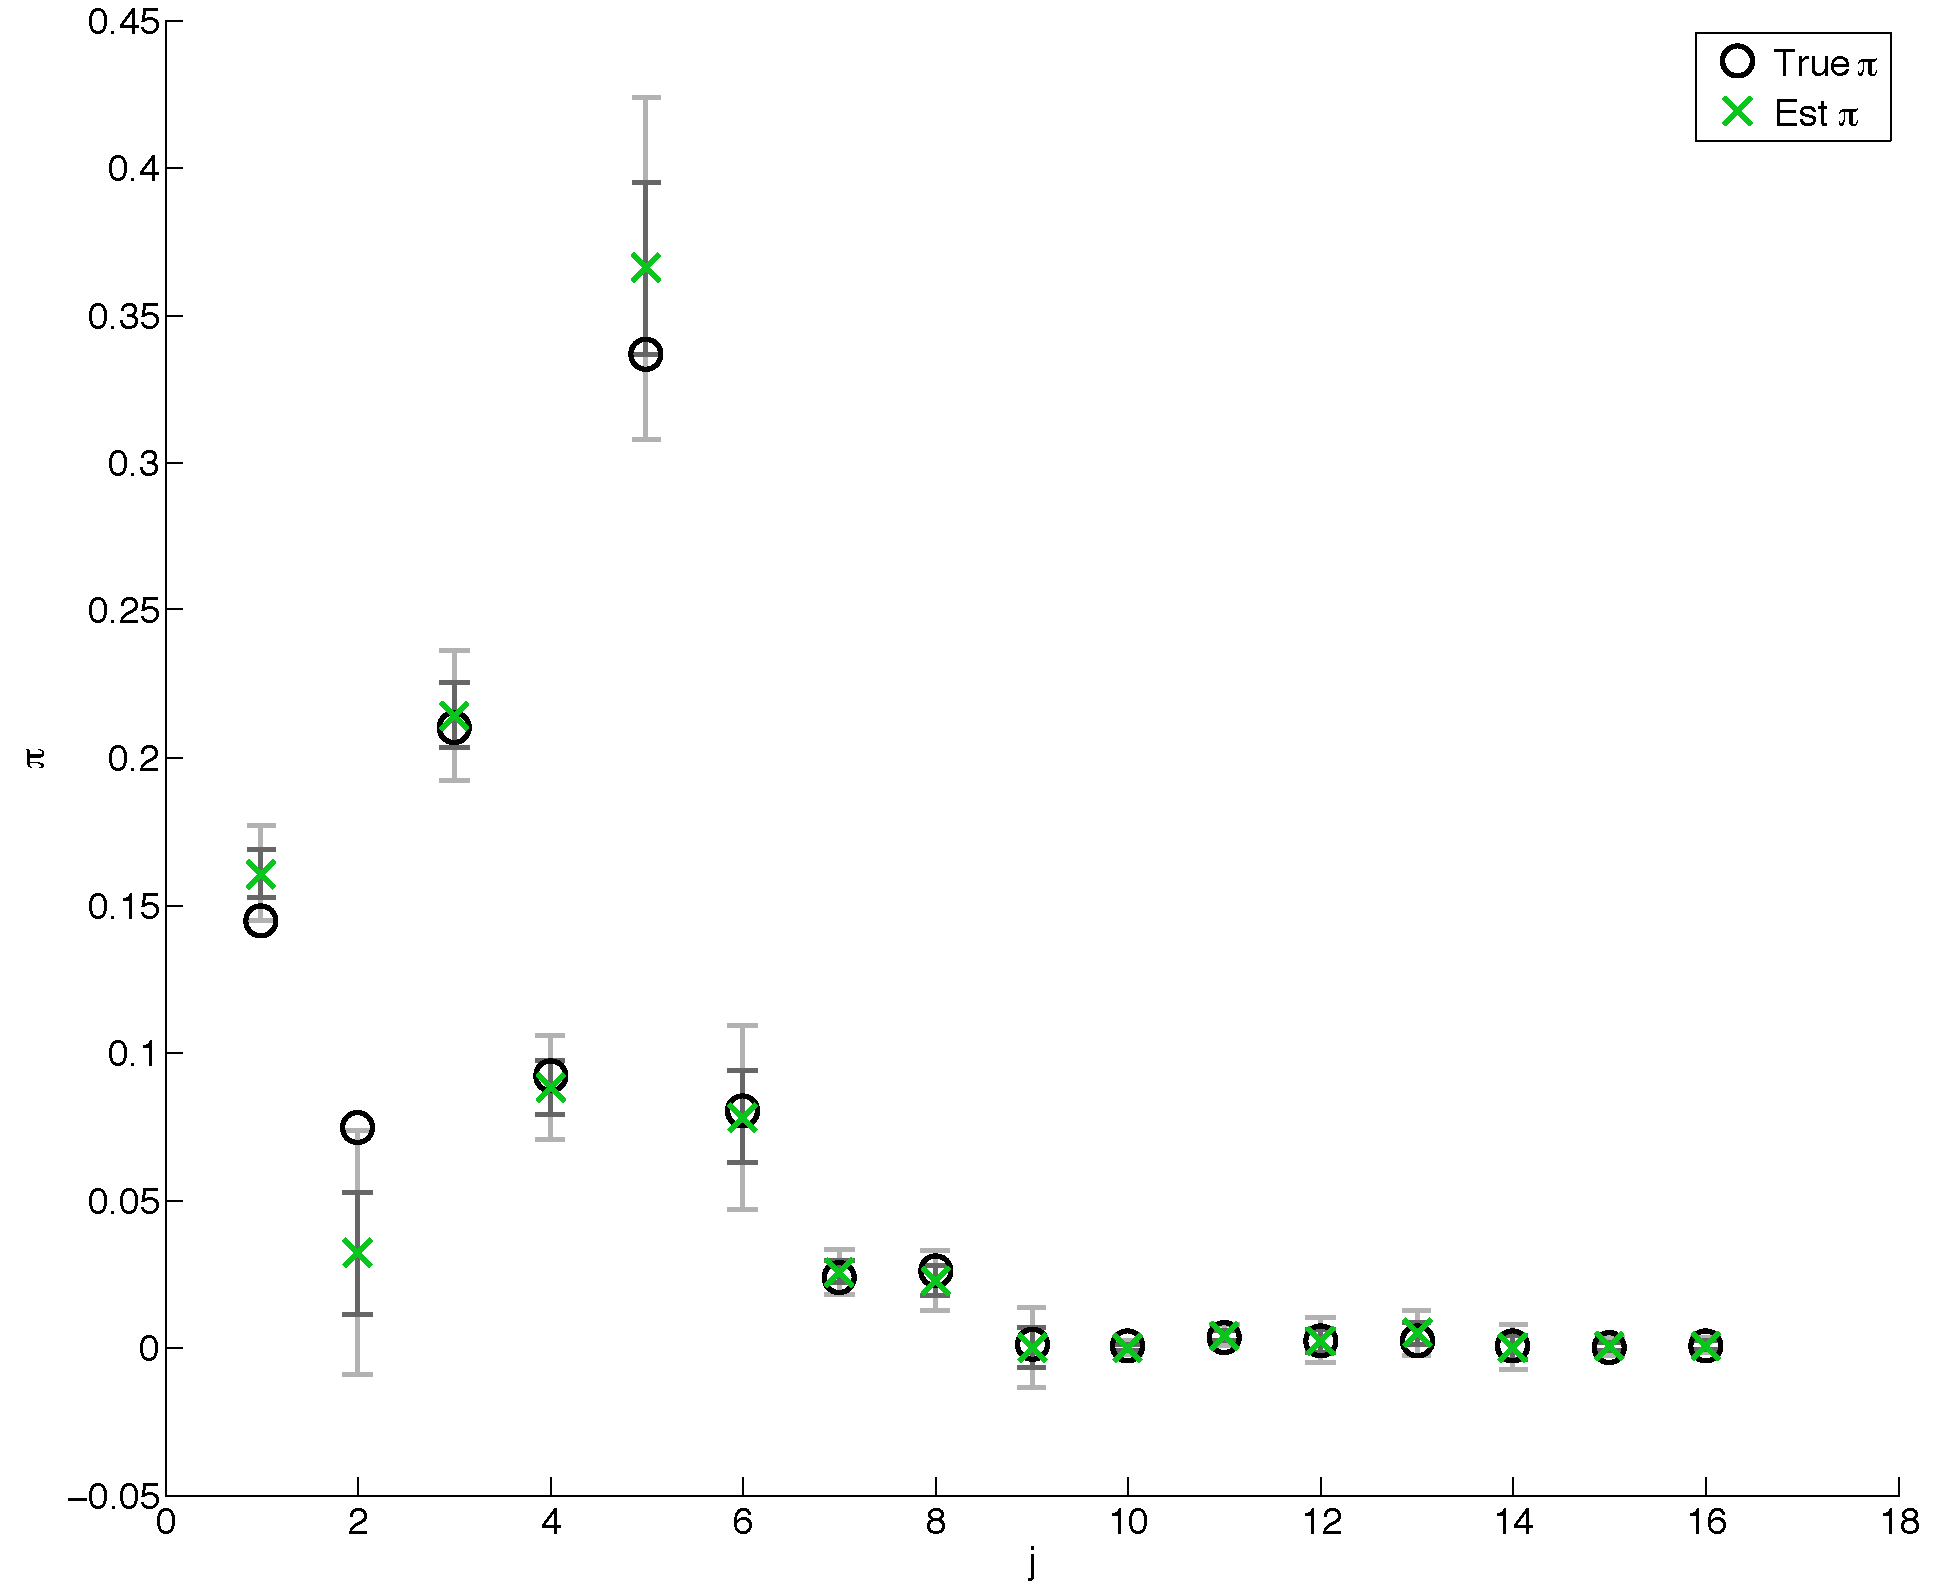
\includegraphics[scale=0.3]{5x5eb.pdf}
			\end{center}
	\end{figure}
	
\end{frame}
%---------------------------------------------------------------------------------------------------------------------------------------------------------------------------
\begin{frame}[shrink]{Confidence Intervals}
	
	\begin{itemize}
		\item Using m-out-of-n bootstrapping, at a 95\% confidence level, produced similar results
		\item for 5x5 grids the estimates of the mixing proportions were not always inside 2 standard deviations, or the 95\% bootstrapped confidence interval
		\item for 2x2 grids, the estimates are almost always inside 2 standard deviations, or the 95\% bootstrapped confidence interval
	\end{itemize}
	
\end{frame}














%%%%%%%%%%%%%%%%%%%%%%%%%%%%%%%%%%%%%%%%%%%%%%%%%%%%%%%%%%%%%%%
%%%%%%%%%%%%%%%%%%%%%%%%%%%%%%%%%%%%%%%%%%%%%%%%%%%%%%%%%%%%%%%
\begin{frame}{Correlation between $\vp$}	
	
	\begin{figure}
			\begin{center}
				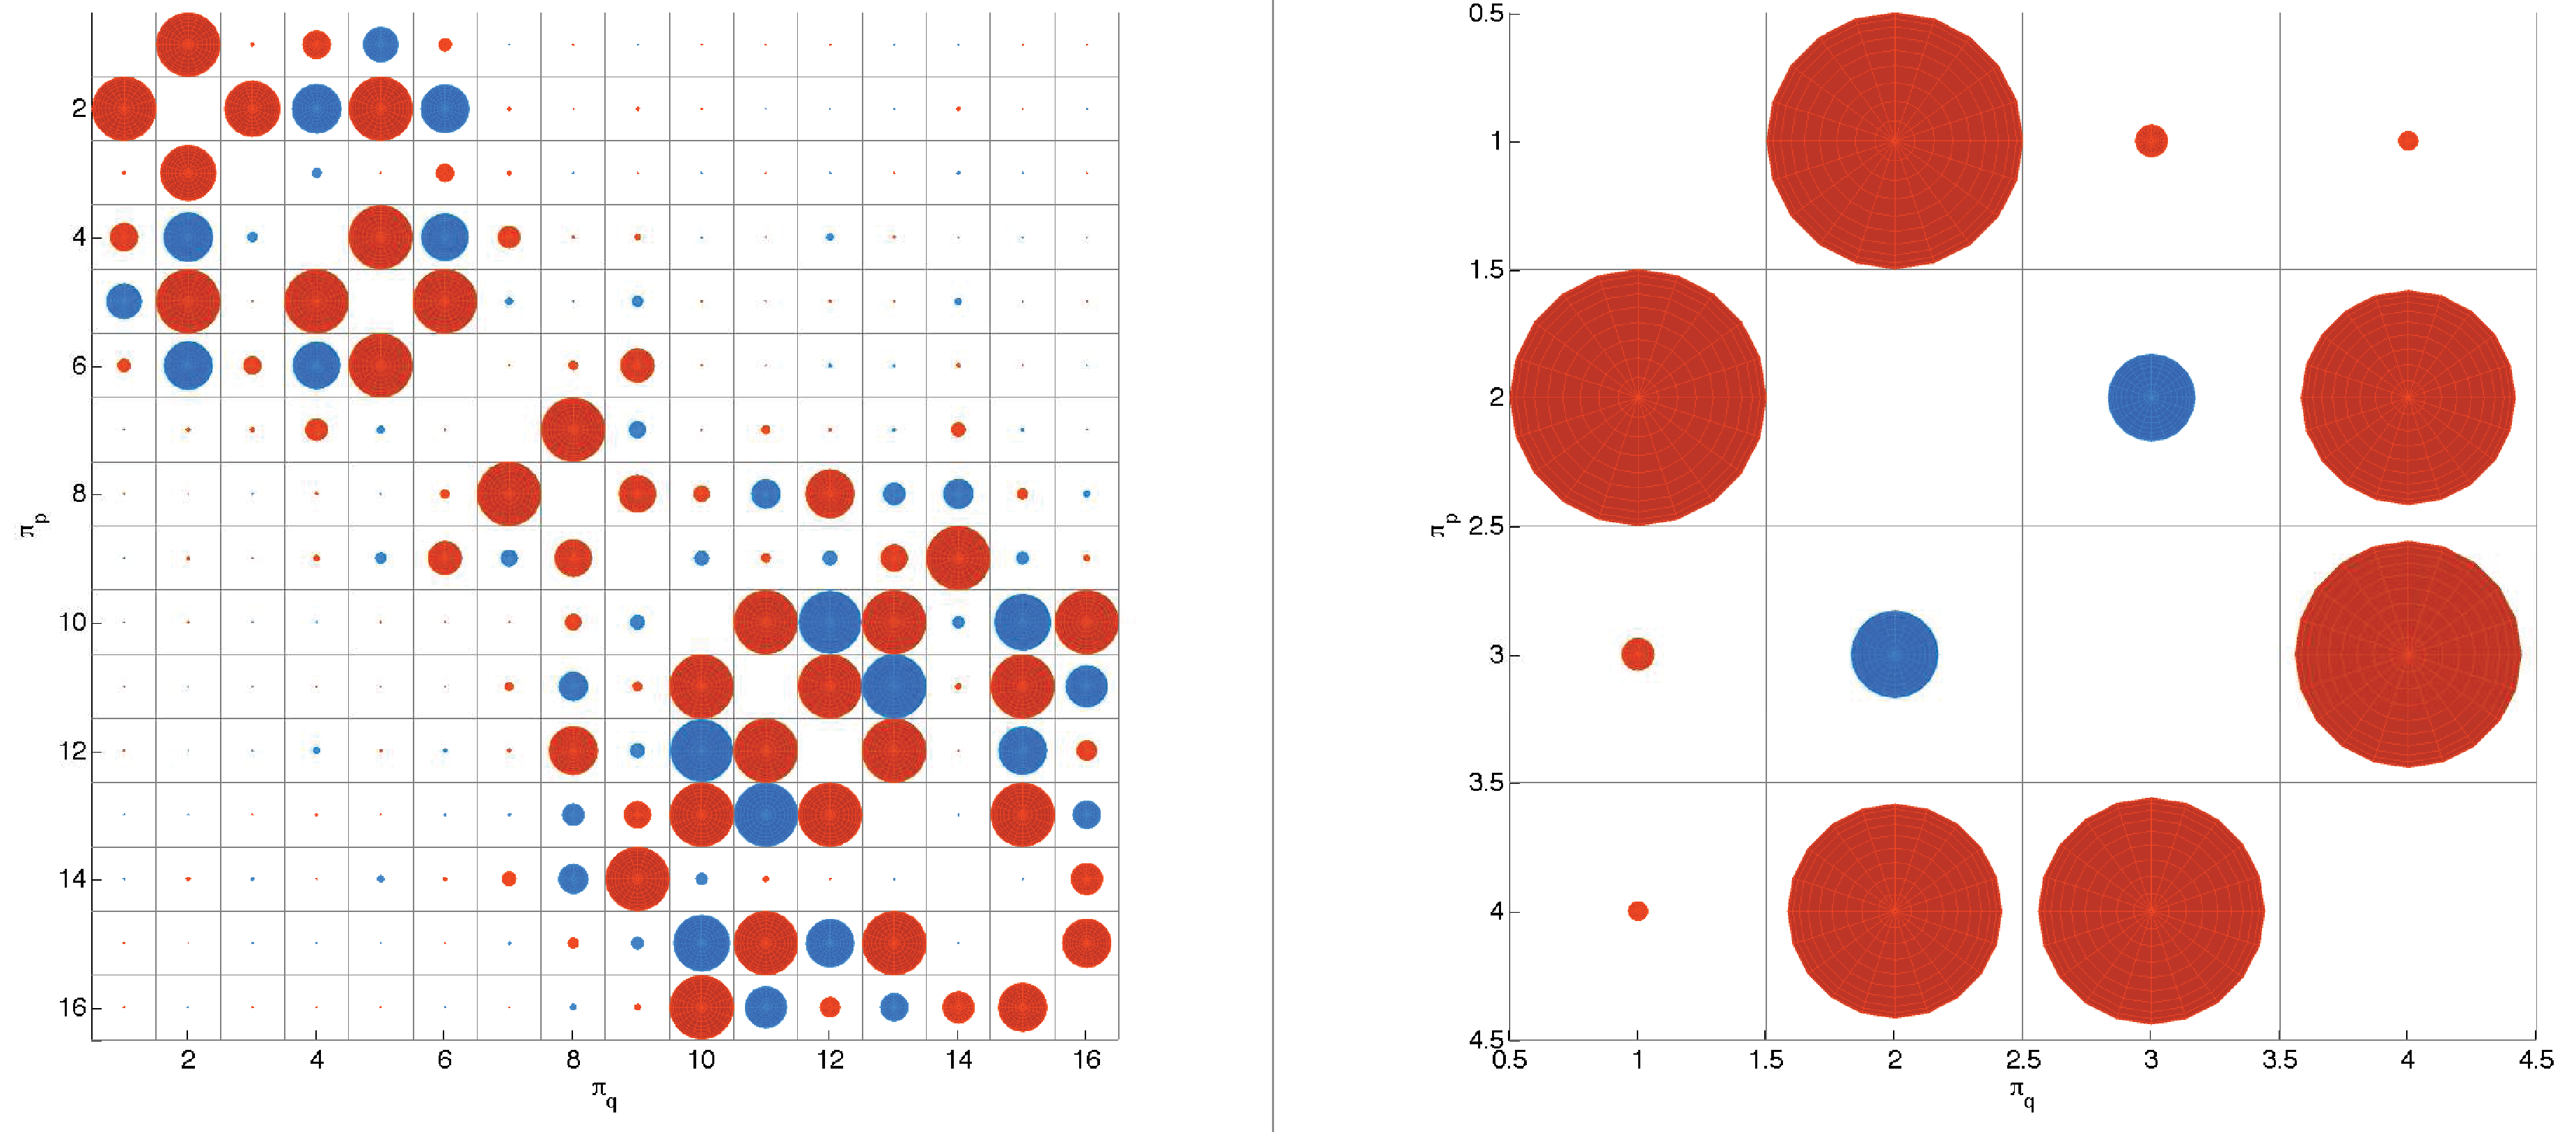
\includegraphics[scale=0.17]{correl.pdf}
			\end{center}
	\end{figure}	
	
\end{frame}
%---------------------------------------------------------------------------------------------------------------------------------------------------------------------------
\begin{frame}[shrink]{Correlation between $\vp$}
	
	\begin{itemize}
		\item larger spheres represent higher values of pi hat
		\item red spheres are negative correlation
		\item blue spheres are positive correlation
		\item mixing components that are right next to eachother, and thus have similar mass and accretion time ranges, tend to have larger correlations.
		\item one way to reduce the correlation might be to produce mixing components on different grids of mass and accretion time
		
		\item Again, m-out-of-n bootstrapping produced similar covariance structures
		
	\end{itemize}
	
\end{frame}












%%%%%%%%%%%%%%%%%%%%%%%%%%%%%%%%%%%%%%%%%%%%%%%%%%%%%%%%%%%%%%%
%%%%%%%%%%%%%%%%%%%%%%%%%%%%%%%%%%%%%%%%%%%%%%%%%%%%%%%%%%%%%%%
\begin{frame}{Conclusion}
	
	Poor results
	\begin{itemize}
		\item 5x5 grids, except in a few cases
		\item Parametric bootstrapping
	\end{itemize}	
	
	
	Good results
	\begin{itemize}
		\item 2x2 grids
		\item EM
		\item 5x5 in a few cases
		\item Confidence intervals
		\begin{itemize}
			\item Observed Fisher information
			\item M-of-n bootstrapping
		\end{itemize}
	\end{itemize}	
	
	
	
	
	Future work
	\begin{itemize}
		\item Adaptive partitioning of mass and time since accretion for mixing components
		\item Smoothing the 1,500 metallicity curves and constructing mixing components from them
	\end{itemize}	
	
\end{frame}
%---------------------------------------------------------------------------------------------------------------------------------------------------------------------------
\begin{frame}[shrink]{Conclusion}
	
	\begin{itemize}
		\item starting with what didn't work
		\item 5x5 grids tended to converge to the wrong answers in all but a handful of cases
		\item since our mixture model is not the true generative model, we can consistently converge on estimates of the mixing proportions that are incorrect.
		\item this is also likely the reason that parametric bootstrapping didn't work--the observed points are not actually generated from a set of mixing components, and so when we make the grid too granular, we find patterns that are not found in the simulated data.
	\end{itemize}	
	\begin{itemize}
		\item we did have success with 2x2 grids
		\item the EM algorithm converged, and we did not see any degeneracies--we always converged on the same answers, even if they weren't the "true" values.
		\item in some cases, the 5x5 grids were fit quite well
		\item m-out-of-n bootstrapping confirmed confidence intervals and covariance matrices derived from observed Fisher information
		
	\end{itemize}
	
	\begin{itemize}
		\item we have done some work on adaptive gridding, based on finding the partitions of mass and time since accretion that maximize the difference between the mixing components, and the underlying metallicity curves
		\item adaptive gridding looks promising, but is still in the early stages
		
		\item since we have 1,500 metallicity curves, we have also investigated smoothing the curves to create 1,500 mixture components
		\item this might increase sensitivity of the algorithm
		\item this approach is also compatible with adaptive gridding
	\end{itemize}
	
\end{frame}



































\end{document}
%%%%%%%%%%%%%%%%%%%%%%%%%%%%%%%%%%%%%%%%%%%%%%%%%%%%%%%%%%%%%%%
%%%%%%%%%%%%%%%%%%%%%%%%%%%%%%%%%%%%%%%%%%%%%%%%%%%%%%%%%%%%%%%
%%%%%%%%%%%%%%%%%%%%%%%%%%%%%%%%%%%%%%%%%%%%%%%%%%%%%%%%%%%%%%%
%%%%%%%%%%%%%%%%%%%%%%%%%%%%%%%%%%%%%%%%%%%%%%%%%%%%%%%%%%%%%%%
%%%%%%%%%%%%%%%%%%%%%%%%%%%%%%%%%%%%%%%%%%%%%%%%%%%%%%%%%%%%%%%
%%%%%%%%%%%%%%%%%%%%%%%%%%%%%%%%%%%%%%%%%%%%%%%%%%%%%%%%%%%%%%%
%%%%%%%%%%%%%%%%%%%%%%%%%%%%%%%%%%%%%%%%%%%%%%%%%%%%%%%%%%%%%%%
%%%%%%%%%%%%%%%%%%%%%%%%%%%%%%%%%%%%%%%%%%%%%%%%%%%%%%%%%%%%%%%
%%%%%%%%%%%%%%%%%%%%%%%%%%%%%%%%%%%%%%%%%%%%%%%%%%%%%%%%%%%%%%%
%%%%%%%%%%%%%%%%%%%%%%%%%%%%%%%%%%%%%%%%%%%%%%%%%%%%%%%%%%%%%%%
%%%%%%%%%%%%%%%%%%%%%%%%%%%%%%%%%%%%%%%%%%%%%%%%%%%%%%%%%%%%%%%
%%%%%%%%%%%%%%%%%%%%%%%%%%%%%%%%%%%%%%%%%%%%%%%%%%%%%%%%%%%%%%%
%%%%%%%%%%%%%%%%%%%%%%%%%%%%%%%%%%%%%%%%%%%%%%%%%%%%%%%%%%%%%%%
%%%%%%%%%%%%%%%%%%%%%%%%%%%%%%%%%%%%%%%%%%%%%%%%%%%%%%%%%%%%%%%





































\begin{frame}[shrink]{A generative finite mixture model}
	
	\alert{hello}
	
	\structure{hello}
	
	\pgfputat{\pgfxy(0,-6.5)}{\pgfbox[left,base]{\pgfimage[width=\textwidth]{denstoobs}}}
	
	\begin{itemize}
		\item \clr{red}{a}bc
	\end{itemize}
	
	\eqn{
		\Bigg[\feh,\afe\Bigg]_{i=1}^{N} \text{i.i.d} \sim f(\alert{x},\structure{y}) = \sum^m_{j=1} \pi_j f_j(x,y)
	}
	
\end{frame}




\begin{frame}{Rigid body dynamics}
	
	\tikzstyle{na} = [baseline=-.5ex]
			
			A modest attempt at using PGF/TikZ. \\
		Green's Theorem: \\
		\begin{itemize}
		\item
		Curl \tikz\node[fill=yellow!20,draw,circle] (n4){};
		\item
		Divergence \tikz\node[fill=green!20,draw,circle] (n2){};
		\end{itemize}
		\begin{equation}
		\oint_{\tikz[baseline]{\node[fill=red!20,anchor=base] (t1) {$\partial D$};}} \,
		\tikz[baseline]{\node[fill=green!20,anchor=base] (t2) {$F\cdot ds$};}
		\ = \
		\int\int_{\tikz[baseline]{\node[fill=blue!20,anchor=base] (t3) {$D$};}} \,(
		\tikz[baseline]{\node[fill=yellow!20,anchor=base] (t4) {$\nabla \times F$};})\cdot k \,dA
		\end{equation}
		\begin{itemize}
		\item
		Boundary of Region \tikz\node[fill=red!20,draw,circle] (n1){};
		\item
		Region \tikz\node[fill=blue!20,draw,circle] (n3){};
		\end{itemize}
		\begin{tikzpicture}[overlay]
		\path[->] (n1) edge [out=90, in=-90] (t1);
		\path[->] (n2) edge [bend left] (t2);
		\path[->] (n3) edge [out=0, in=-90] (t3);
		\path[->] (n4) edge [out=0, in=90] (t4);
		\end{tikzpicture}
	\end{frame}









%%%%%%%%%%%%%%%%%%%%%%%%%%%%%%%%%%%%%%%%%%%%%%%%%%%%%%%%%%%%%%%
%%%%%%%%%%%%%%%%%%%%%%%%%%%%%%%%%%%%%%%%%%%%%%%%%%%%%%%%%%%%%%%
\begin{frame}{EM formation history for $m$=25}
	
	\begin{figure}
			\begin{center}
				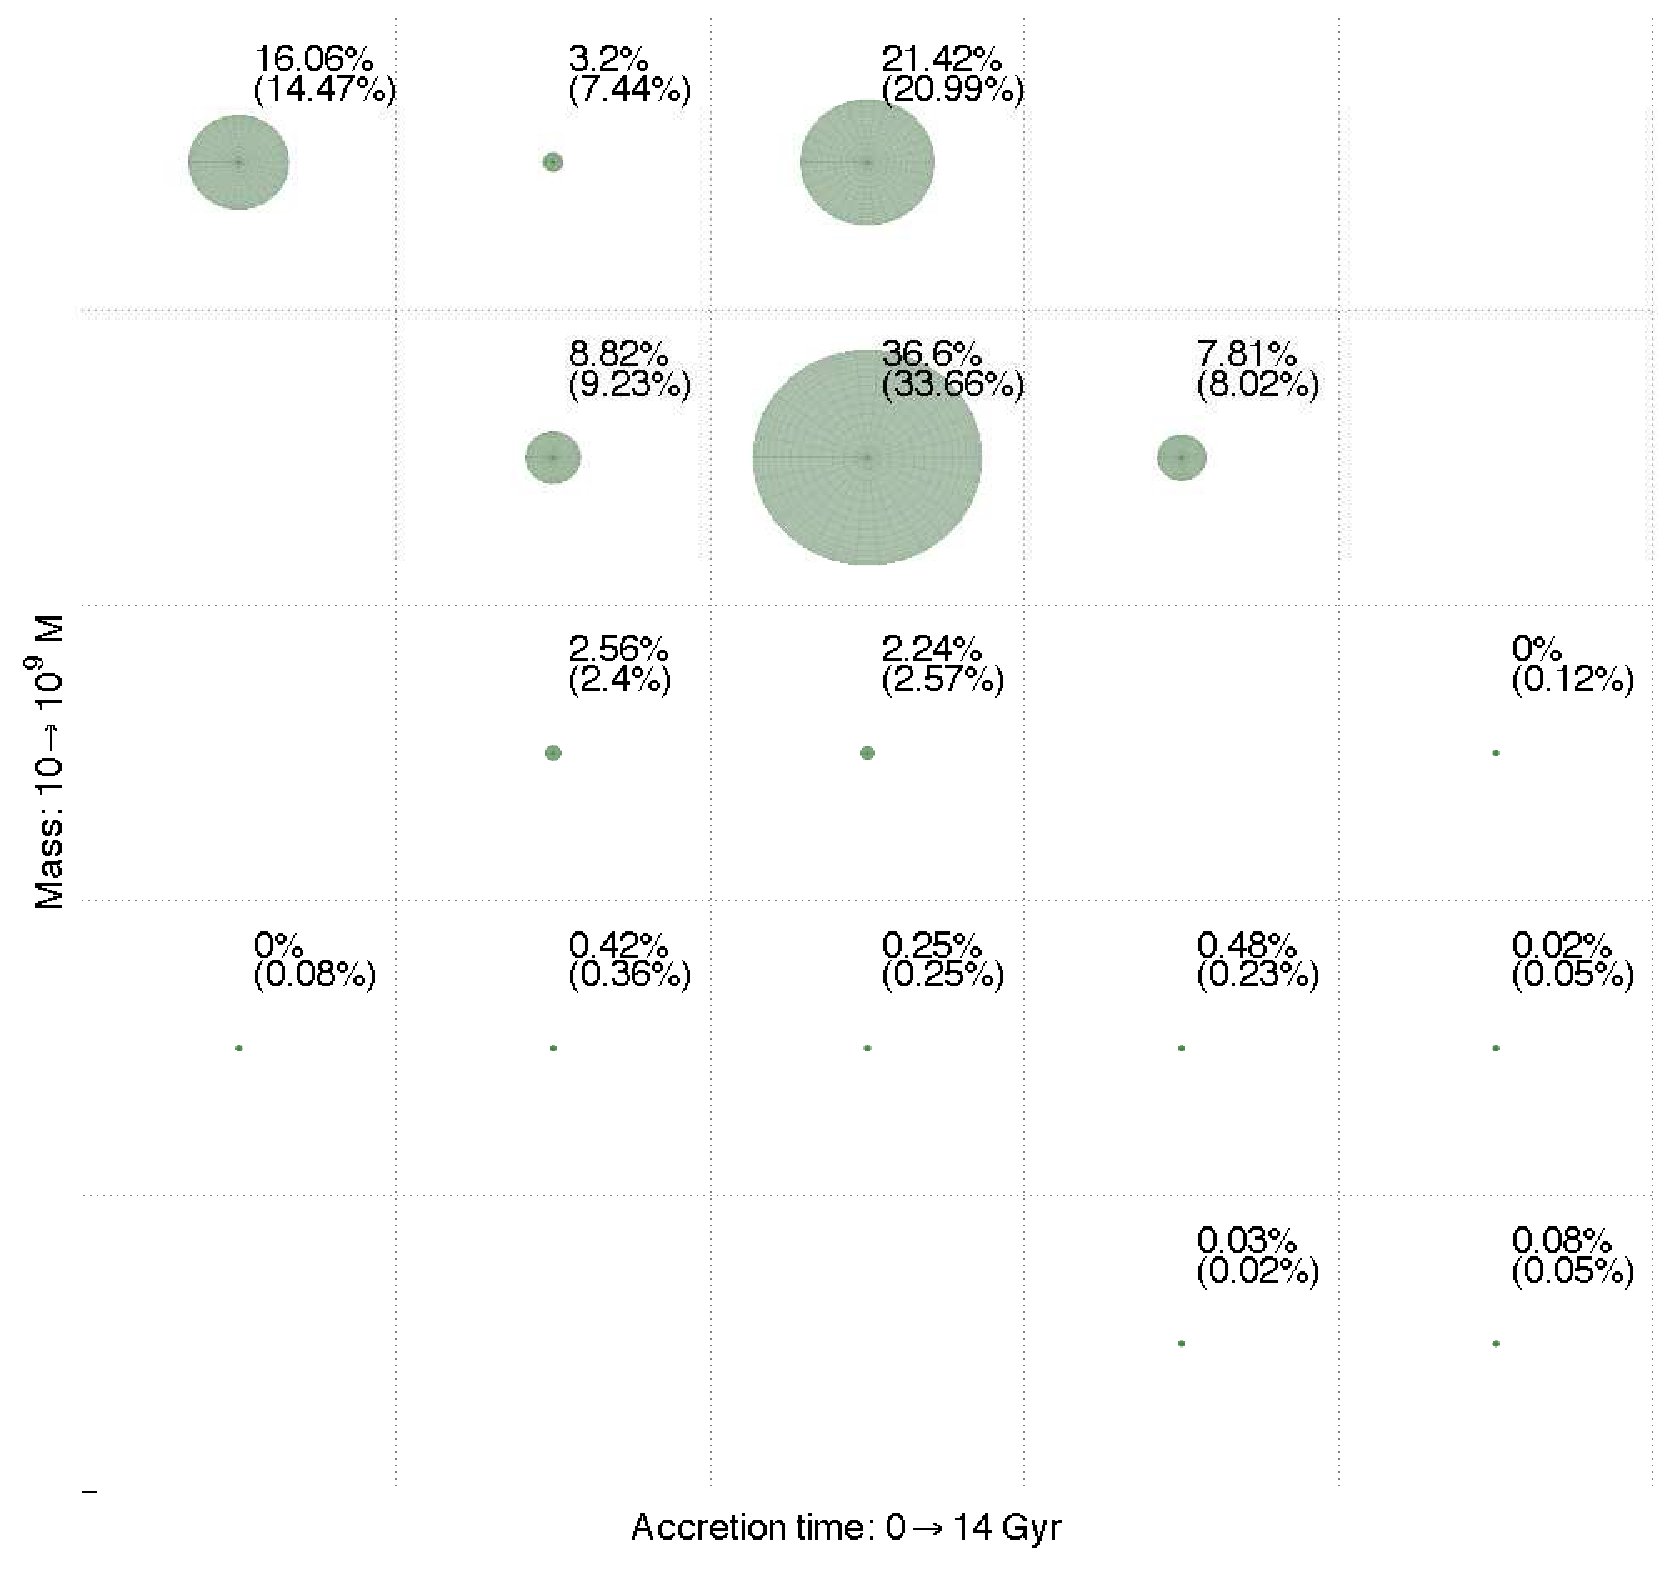
\includegraphics[scale=0.3]{h3fh.pdf}
			\end{center}
	\end{figure}
	
\end{frame}












%%%%%%%%%%%%%%%%%%%%%%%%%%%%%%%%%%%%%%%%%%%%%%%%%%%%%%%%%%%%%%%
%%%%%%%%%%%%%%%%%%%%%%%%%%%%%%%%%%%%%%%%%%%%%%%%%%%%%%%%%%%%%%%
\begin{frame}{EM formation history for $m$=4}
	
	\begin{figure}
			\begin{center}
				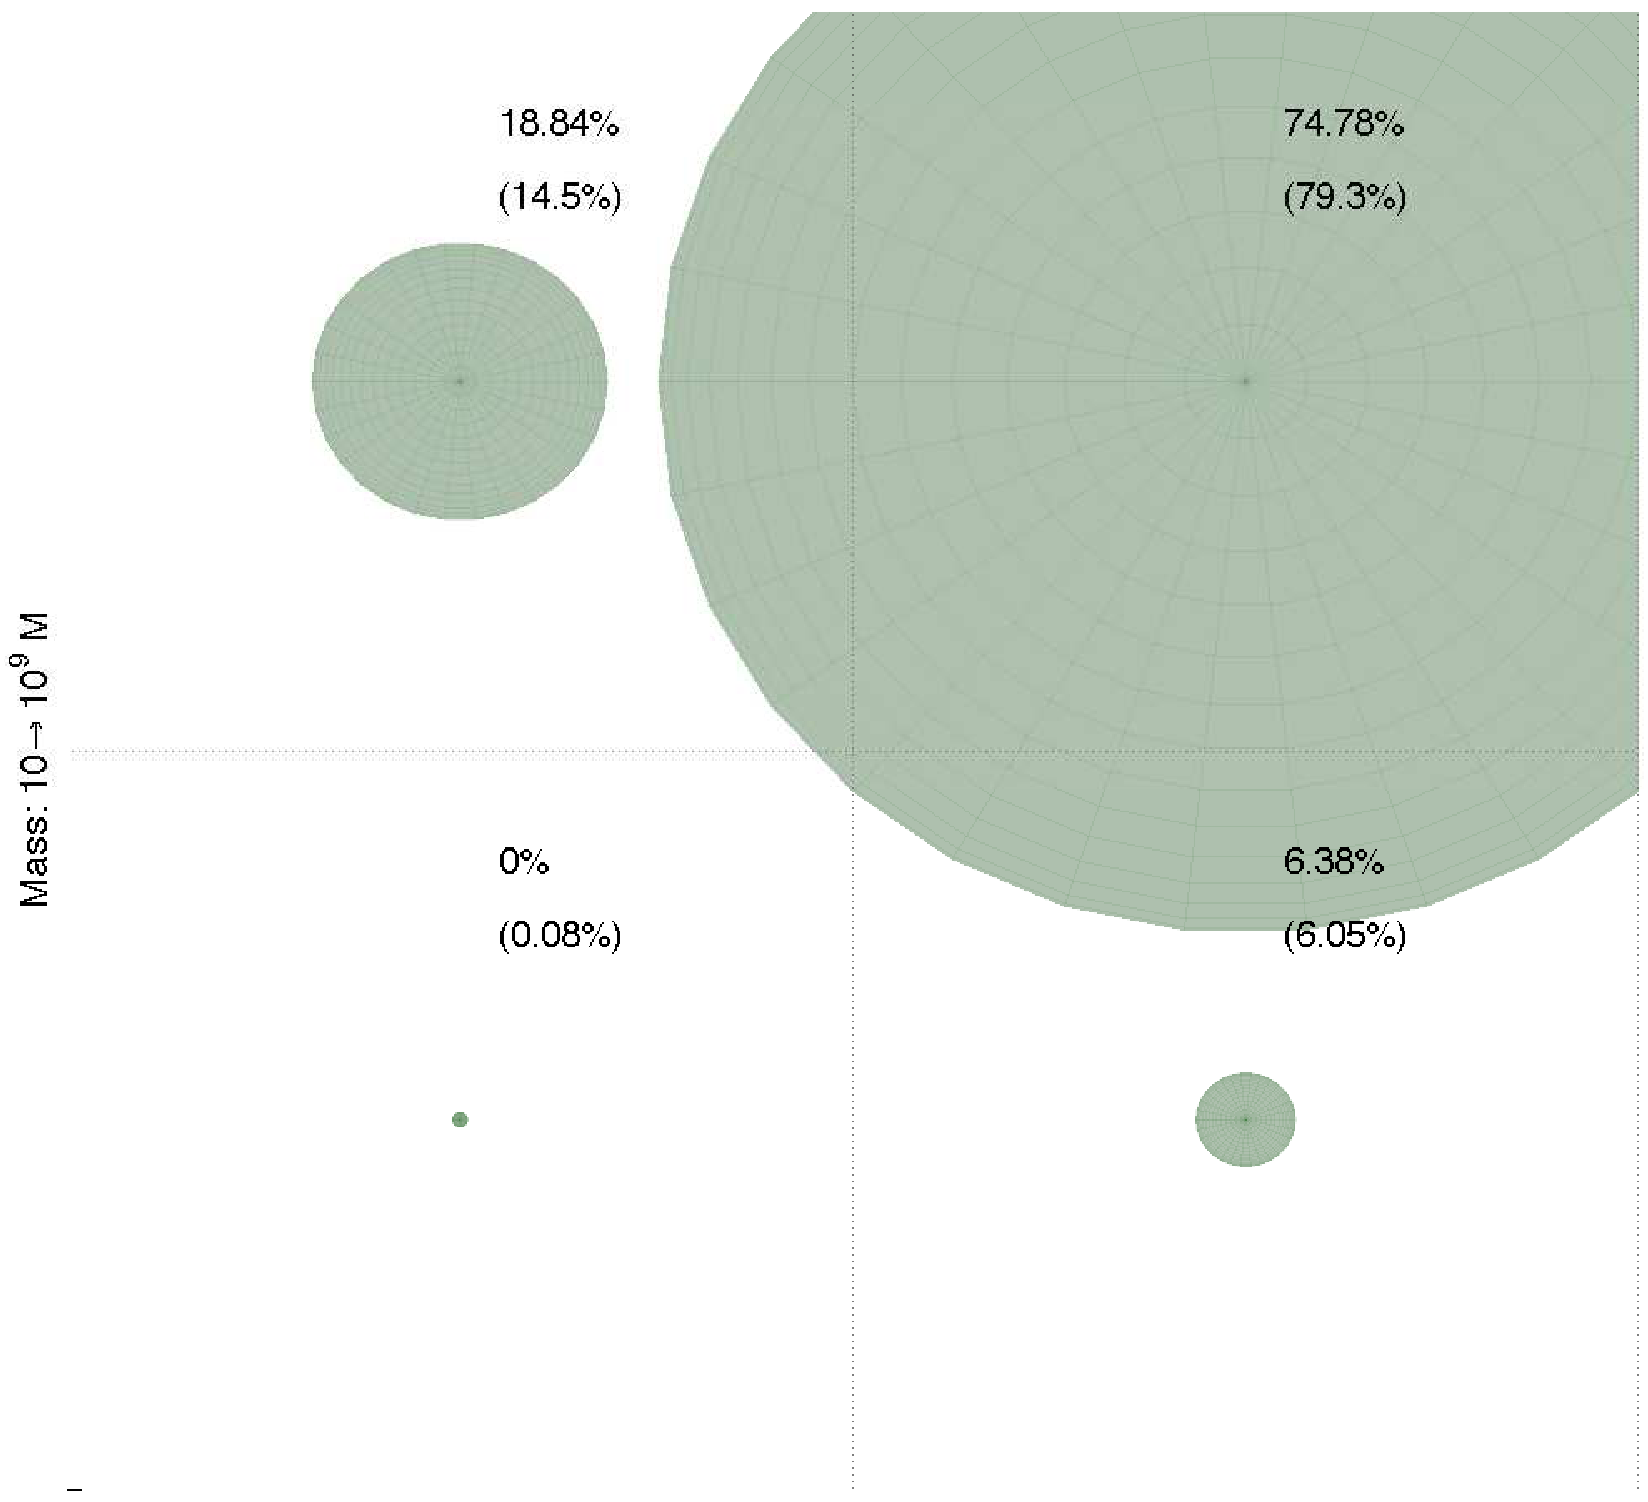
\includegraphics[scale=0.3]{fh2x2.pdf}
			\end{center}
	\end{figure}

	
\end{frame}












